%% Algèbre
\newcommand{\AS}[1]{\mathcal{#1}}  % la police des polynômes d'AS
\newcommand{\biv}[1]{\mathfrak{#1}}  % la police des polynomes bivariés
\newcommand{\vect}[1]{\vec{#1}}  % la police des vecteurs colonne
\newcommand{\bs}{\mathbf{s}}  % s boldface
\newcommand{\bC}{\mathbf{C}}  % C boldface
\newcommand{\bB}{\mathbf{B}}  % B boldface
\newcommand{\bD}{\mathbf{D}}  % D boldface
\newcommand{\bP}{\mathbf{P}}  % D boldface

\newcommand{\sC}{\mathsf{K}}  % K sans serif -- used to clash with ModComp
\renewcommand{\L}{\mathsf{L}}  % L sans serif

\part{Change of order in triangular sets}

\chapter{Summary}
In this chapter we give fast algorithms for arithmetic operations in
Artin-Schreier towers. Prior results for this task are due to
Cantor~\cite{cantor89} and Couveignes~\cite{couveignes00}. However,
the algorithms of~\cite{couveignes00} need as a prerequisite a fast
multiplication algorithm in some towers of a special kind, called
``Cantor towers'' in~\cite{couveignes00}. Such an algorithm is
unfortunately not in the literature, making the results
of~\cite{couveignes00} non practical. This chapter fills the gap.

To our knowledge, no previous work provided the missing ingredients to
put Couveignes' algorithms to practice. Part of Cantor's results were
independently discovered by Wang and Zhu~\cite{wang+zhu88} and have
been extended in another direction (fast polynomial multiplication
over arbitrary finite fields) by von zur Gathen and
Gerhard~\cite{vzgatehn+gerhard02} and Mateer~\cite{mateer08}.

Technically, the main algorithmic contribution of this chapter is a
fast chan\-ge-of-basis algorithm based on the techniques of
Chapter~\ref{cha:trace-computations}. Building on this, it is possible
to obtain fast multiplication routines, and by extension completely
explicit versions of all algorithms of~\cite{couveignes00}. Along the
way, we also extend constructions of Cantor to the case of a general
finite base field $\U_0$, where Cantor had $\U_0=\F_p$.

The algorithms presented in this chapter have been integrated in a
\texttt{C++} library called \texttt{FAAST}, based on Shoup's
\texttt{NTL}~\cite{shoup2003ntl} library. This chapter is joint work
with Schost~\cite{df+schost09}.


\section{Introduction}
\label{sec:artin-schr-extens}

If $\U$ is a field of characteristic $p$, polynomials of the form
\begin{equation}
  \label{eq:36}
  X^p - X - \alpha
  \text{,}  
\end{equation}
with $\alpha \in \U$ are called {\em Artin-Schreier polynomials}; a
field extension $\U'/\U$ is {\em Artin-Schreier} if it is of the form
$\U' = \U[X]/P$, with $P$ an Artin-Schreier polynomial.

An {\em Artin-Schreier tower} of height $k$ is a sequence of
Artin-Schreier extensions $\U_i / \U_{i-1}$, for $1\le i \le k$; it is
denoted by $(\U_0, \ldots, \U_k)$. In what follows, we only consider
extensions of finite degree over $\F_p$. Thus, $\U_i$ is of degree
$p^i$ over $\U_0$, and of degree $p^id$ over $\F_p$, with
$d=[\U_0:\F_p]$.

The importance of this concept comes from the fact that all Galois
extensions of degree $p$ are Artin-Schreier (see \cite[VI,
$\S6$]{lang}). As such, they arise frequently, e.g., in number theory
(for instance, when computing $p^k$-torsion groups of Abelian
varieties over $\F_p$). The need for fast arithmetics in these towers
is motivated in particular by applications to isogeny computation and
point-counting in cryptography, as we will see in
Chapter~\ref{cha:algor-small-char}.

We count all time complexities in number of operations in
$\F_p$. Then, notation being as before, optimal algorithms in $\U_k$
would have complexity $O(p^kd)$; most of our results are (up to
logarithmic factors) of the form $O(p^{k+\alpha} d^{1+\beta})$, for
small constants $\alpha,\beta$ such as $0,1,2$ or $3$.

For several operations, different algorithms will be available, and
their relative efficiencies can depend on the values of $p$, $d$ and
$k$. In these situations, we always give details for the case where
$p$ is small, since cases such as $p=2$ or $p=3$ are especially useful
in practice. Some of our algorithms could be slightly
improved, but we usually prefer giving the simpler solutions.

In the following section we give the relevant definitions, and
preliminaries. In Section~\ref{sec:fast-tower}, we define a specific
Artin-Schreier tower, where arithmetic operations will be fast. Our
key change-of-basis algorithm for this tower is in
Section~\ref{sec:level-embedding}. In
Sections~\ref{sec:pseudotrace-frobenius}
and~\ref{sec:couveignes-algorithm}, we revisit Couveignes' algorithm
for isomorphism between Artin-Schreier towers~\cite{couveignes00} in
our context, which yields fast arithmetics for {\em any}
Artin-Schreier tower. Finally, Section~\ref{sec:artin-benchmarks} presents
our implementation of the \texttt{FAAST} library and gives
experimental results.



% Local Variables:
% mode:flyspell
% ispell-local-dictionary:"american"
% mode: TeX-PDF
% mode: reftex
% TeX-master: "../these"
% End:
%
% LocalWords:  Schreier Artin pseudotrace frobenius bivariate memoization
% LocalWords:  isogeny Couveignes


\chapter{Standard techniques}
\section{Gröbner bases}
\section{Resultants}
\section{The case of finite fields}


\chapter{Trace formulae}
\section{Rouiller's algorithm}
\section{Shoup's algorithm}
\section{Pascal-Schost algorithm}

\chapter{The Artin-Schreier case}
\section{Preliminaries}
\label{sec:arithmetics}

As a general rule, variables and polynomials are in upper
case; elements algebraic over $\F_p$ (or some other field, that will
be clear from the context) are in lower case.
 
%%%%%%%%%%%%%%%%%%%%%%%%%%%%%%%%%%%%%%%%%%%%%%%%%%%%%%%%%%%%

\subsection{Element representation}\label{ssec:rep}

We let $Q_0$ be in $\F_p[X_0]$ and $\U_0=\F_p[X_0]/Q_0$.

\begin{definition}
  \label{def:primitive-tower}
  Let $(G_i)_{0 \le i < k}$ be a sequence of polynomials over $\F_p$,
  with $G_i$ in $\F_p[X_0,\dots,X_i]$.  The sequence $(G_i)_{0\le i
    <k}$ is said to {\em define the tower} $(\U_0,\dots,\U_k)$ if for
  $i \ge 0$, $\U_i=\F_p[X_0,\dots,X_i]/K_i$, where $K_i$ is the ideal
  generated by
  \begin{equation}
    \label{eq:57}
    \left | \begin{array}{l}
        P_i=X_i^p-X_i -G_{i-1}(X_0,\dots,X_{i-1})\\
        ~~~\,~\vdots\\
        P_1=X_1^p-X_1-G_0(X_0)\\
        Q_0(X_0)
      \end{array}\right .
  \end{equation}
  in $\F_p[X_0,\dots,X_i]$, and if $\U_i$ is a field. 

  The residue class of $X_i$ (resp. $G_i$) in $\U_i$, and thus in
  $\U_{i+1},\dots$, is written $x_i$ (resp. $\gamma_i$), so that we
  have $x_i^p-x_i=\gamma_{i-1}$.
\end{definition}

Finding a suitable $\F_p$-basis to represent elements of a tower
$(\U_0,\dots,\U_k)$ is a crucial question. 

\begin{definition}[Multivariate basis]
  If $d=\deg(Q_0)$, the \emph{multivariate basis} $\basis{B}_i$ of
  $\U_i$ is
  \begin{equation}
  \basis{B}_i=
  \{x_0^{e_0} \cdots x_i^{e_i} \;|\; 0 \le e_0 < d,\; 0\le e_j < p 
  \text{ for $j>0$}\}
  \text{.}
\end{equation}
\end{definition}

However, in this basis, we do not have very efficient arithmetic
operations, starting from multiplication. Indeed, the natural approach
to multiplication in $\basis{B}_i$ consists in a polynomial multiplication,
followed by reduction modulo $(Q_0,P_1,\dots,P_i)$; however, the
initial product gives a polynomial of partial degrees
$(2d-2,2p-2,\dots,2p-2)$, so the number of monomials appearing is not
linear in $[\U_i:\F_p]=p^id$.  See~\cite{li+moreno+schost07} for
details.

As a workaround, we introduce the notion of a {\em primitive tower}.

\begin{definition}[Primitive tower]
  \pdfmctwo{Link to previous definition, to avoid ambiguities on xi.}
  With the same notation of Definition~\ref{def:primitive-tower}, a
  tower $(\U_0,\ldots,\U_k)$ defined by $(G_i)_{0 \le i < k}$ is said
  to be \emph{primitive} if
  \begin{equation}
    \label{eq:59}
    \U_i = \F_p[x_i]
  \end{equation}
  for all $i$. In this case, we let $Q_i\in \F_p[X]$ be the minimal
  polynomial of $x_i$, of degree $p^id$.
\end{definition}

\begin{definition}[Univariate basis]
  Let $(\U_0,\ldots,\U_k)$ be a primitive tower, the \emph{univariate
    basis} $\basis{C}_i$ of $\U_i$ is the $\F_p$-basis
  \begin{equation}
    \pdfmctwo{Explicit indices for the basis.}
    \basis{C}_i=\{x_i^a \;|\; 0\le a<p^id\}
    \text{.}  
  \end{equation}
  To stress the fact that $v\in\U_i$ is represented on the univariate
  basis, we write $v\wrt\U_i$.
\end{definition}

In a primitive tower, unless otherwise stated, we represent the
elements of $\U_i$ on the univariate basis. In this basis, assuming
$Q_i$ is known, additions and subtractions are done in time $p^id$,
multiplications in time $O(\Mult(p^id))$ and inversions in time
$O(\Mult(p^id)\log(p^id))$ (see Section~\ref{sec:fund-algor}).

Remark that having fast arithmetic operations in $\U_i$ enables us to
write fast algorithms for polynomial arithmetic in $\U_i[Y]$, where
$Y$ is a new variable. Extending the previous notation, let us write
$A \wrt\U_i[Y]$ to indicate that a polynomial $A \in \U_i[Y]$ is
written on the basis $(x_i^\alpha Y^\beta)_{0 \le \alpha < p^id, 0 \le
  \beta}$ of $\U_i[Y]$.  Then, given $A,B \wrt \U_i[Y]$, both of
degrees less than $n$, one can compute $AB \wrt \U_i[Y]$ in time
$O(\Mult(p^id n))$ using Kronecker's substitution (see
Section~\ref{sec:mult-polyn}).

One can extend the fast Euclidean division algorithm to this context,
as Newton iteration reduces Euclidean division to polynomial
multiplication (see Section~\ref{sec:newtons-iteration}). This implies
that Euclidean division of a degree $n$ polynomial $A \wrt \U_i[Y]$ by
a monic degree $m$ polynomial $B \wrt \U_i[Y]$, with $m \le n$, can be
done in time $O(\Mult(p^id n))$.

Finally, fast GCD techniques carry over as well, as they are based on
multiplication and division. As we saw in
Section~\ref{sec:eucl-algor-rati}, the extended GCD of two monic
polynomials $A,B \wrt \U_i[Y]$ of degree at most $n$ can be computed
in time $O(\Mult(p^id n \log(n)))$.

%%%%%%%%%%%%%%%%%%%%%%%%%%%%%%%%%%%%%%%%%%%%%%%%%%%%%%%%%%%%

\subsection{Trace and pseudotrace}\label{ssec:tpt}


We continue with a few useful facts on traces.

\begin{proposition}
  We have the following well-known properties:
  \begin{align}
  \tag{$\mathbf{P}_1$}\label{eq:78} &\begin{array}{c}  
  \Tr_{\F_{q^n}/\F_q}: a \mapsto \sum_{\ell=0}^{n -
    1}a^{q^\ell} \text{,}
  \end{array}\\
  \tag{$\mathbf{P}_2$}\label{eq:trcomp}
  &\Tr_{\F_{q^{mn}}/\F_q} = \Tr_{\F_{q^m}/\F_q} \circ
  \Tr_{\F_{q^{mn}}/\F_{q^m}}\text{.}
\end{align}
\end{proposition}
\begin{proof}
  This is a direct consequence of
  Proposition~\ref{th:basic-galois-theory:trace}.
\end{proof}

\begin{proposition}
  \label{th:p3}
  If $\U'/\U$ is an Artin-Schreier extension generated by a polynomial
  $Q$ and $x$ is a root of $Q$ in $\U'$, then
\begin{equation}
  \tag{$\mathbf{P}_3$}\label{eq:pd} \Tr_{\U'/\U}(x^j) = 0~ \text{for}~j
  <p-1; \quad \Tr_{\U'/\U}(x^{p-1}) = -1\text{.}
\end{equation}
\end{proposition}
\begin{proof}
  This is a consequence of Lemma~\ref{th:multi-newton-sums}. In fact
  \begin{equation}
    \sum_{i\ge0} \frac{\Tr(x^{i})}{T^{i+1}} = \frac{Q'(T)}{Q(T)} =
    -\frac{1}{T^p-T-\alpha}
    \text{,}
  \end{equation}
  from which we deduce
  \begin{align}
    \label{eq:61}
    &\Tr(x^i) = 0 &\text{for $0\le i<p-1$,}\\
    &\Tr(x^{p-1}) - \Tr(1) = \Tr(x^{p-1}) = -1\text{,}\\
    &\Tr(x^{i+p}) - \Tr(x^{i+1}) - \alpha\Tr(x^{i}) = 0 &\text{for $i\ge 0$.}
  \end{align}
\end{proof}

\begin{proposition}
  \label{th:artin-schreier}
  The Artin-Schreier polynomial $X^p-X-\alpha$ is irreducible in $\F_q$
  if and only if
  \begin{equation}
    \label{eq:62}
    \Tr_{\F_q/\F_p}(\alpha) \ne 0
    \text{.}
  \end{equation}
  If it is reducible, then it is split and its roots are 
  \begin{equation}
    \label{eq:63}
    \eta, \eta+1, \ldots, \eta + p -1
    \text{.}
  \end{equation}
\end{proposition}
\begin{proof}
  This proof is from \cite[Chapter~2]{lidl+niederreiter:2}.

  Since $p$ is prime, $X^p-X-\alpha$ is either irreducible or
  split. In the second case, Eq.~\eqref{eq:63} is obvious.

  Suppose it is split and let $\eta$ be one of its roots. Then
  \begin{equation}
    \Tr_{\F_q/\F_p}(\alpha) = \Tr_{\F_q/\F_p}(\eta^p) - \Tr_{\F_q/\F_p}(\eta) = 0
    \text{,}
  \end{equation}
  where the last equality comes from
  \ref{th:basic-galois-theory:trace}.

  Suppose now that $\Tr_{\F_q/\F_p}(\alpha)=0$, and let $\eta$ be a
  root of $X^p-X-\alpha$ in its splitting field. Let $m=[\F_q:\F_p]$,
  then by \eqref{eq:78}
  \begin{equation}
    0=\Tr_{\F_q/\F_p}(\alpha) = \sum_{i=0}^{m-1}\alpha^{p^i} =
    \sum_{i=0}^{m-1}(\eta^p-\eta)^{p^i} =\eta^{q}-\eta
    \text{,}
  \end{equation}
  thus $\eta\in\F_q$.
\end{proof}

\pdfmcone{Linked to section 2.2.4.}
Following~\cite{vzgathen+shoup92,couveignes00}, we also use a
generalization of the trace, as already introduced in
Section~\ref{sec:comp-frob-trace}.

\begin{definition}[Pseudotrace]
  The $n$-th {\em pseudotrace} of order $m$ is the
  $\F_{p^m}$-linear operator
  \begin{equation*}
    \PTr_{(n,m)}: a \mapsto \sum_{\ell=0}^{n-1}a^{p^{m\ell}}
    \text{;}
  \end{equation*}
  for $m=1$, we call it the $n$-th pseudotrace and write $\PTr_n$.
\end{definition}

\begin{nota}
  \pdfmctwo{Slightly more precise on
    where v lives.}  In our context, for $n=[\U_i:\U_j]=p^{i-j}$ and
  $m=[\U_j:\F_p]=p^jd$, $\PTr_{(n,m)}(v)$ coincides with
  $\Tr_{\U_{i}/\U_j}(v)$ for $v$ in $\U_i$; however $\PTr_{(n,m)}(v)$
  remains defined for $v$ in a field extension of $\U_i$, whereas
  $\Tr_{\U_{i}/\U_j}(v)$ is not.
\end{nota}


% Local Variables:
% mode:flyspell
% ispell-local-dictionary:"american"
% mode: TeX-PDF
% mode: reftex
% TeX-master: "../these"
% End:
%
% LocalWords:  Schreier Artin pseudotrace frobenius bivariate memoization

%% these.tex
%% Copyright 2010 Luca De Feo
%% All rights reserved


\section{A primitive tower}
\label{sec:fast-tower}

Our first task in this section is to describe a specific
Artin-Schreier tower where arithmetic will be fast; then, we explain
how to construct this tower. 

%%%%%%%%%%%%%%%%%%%%%%%%%%%%%%%%%%%%%%%%%%%%%%%%%%%%%%%%%%%%

\subsection{Definition}

The following theorem extends results by
Cantor~\cite[Theorem~1.2]{cantor89}, who dealt with the case
$\U_0=\F_p$.

\begin{theorem}
  \label{th:cantor}
  Let $\U_0=\F_p[X_0]/Q_0$, with $Q_0$ irreducible of
  degree $d$, let $x_0 = X_0 \bmod Q_0$ and assume that
  $\Tr_{\U_0/\F_p}(x_0)\ne0$. Let $(G_i)_{0 \le i <k}$ be defined by
$$ \begin{cases}
G_0 = ~X_0\\
G_1 = ~X_1        &\text{if $p=2$ and $d$ is odd,}\\
G_i = ~X_i^{2p-1} &\text{in any other case.}
\end{cases}$$
Then, $(G_i)_{0 \le i <k}$ defines a primitive tower $(\U_0,\dots,\U_k)$.
\end{theorem}

As before, for $i \ge 1$, let $P_i = X_i^p - X_i - G_{i-1}$ and for $i
\ge 0$, let $K_i$ be the ideal $\langle Q_0,P_1,\dots,P_i\rangle$ in
$\F_p[X_0,\dots,X_i]$.  Then the theorem says that for $i\ge 0$,
$\U_i=\F_p[X_0,\dots,X_i]/K_i$ is a field, and that $x_i=X_i \bmod
K_i$ generates it over $\F_p$.  We prove it as a consequence of a more
general statement.

\begin{lemma}
  Let $\U$ be the finite field with $p^n$ elements, and let $\U'/\U$
  be an extension field with $[\U':\U]=p^i$. Let $\alpha\in\U'$ be
  such that
  \begin{equation}
    \label{eq:ASgen}
    \Tr_{\U'/\U}(\alpha) = \beta \ne 0
    \text{,}
  \end{equation}
  then $\F_p[\beta]\subset\F_p[\alpha]$ and $p^i$ divides
  $\left[\F_p[\alpha]:\F_p[\beta]\right]$.
\end{lemma}
\begin{proof}
  \pdfmctwo{Recalled what Eq. P2 is.}
  Equation~\eqref{eq:ASgen} can be written as $\beta = \sum_j
  \alpha^{p^{jn}}$, thus $\F_p[\beta] \subset \F_p[\alpha]$.  The rest
  of the proof follows by induction on $i$. If $[\U':\U]=1$, then
  $\alpha=\beta$ and there is nothing to prove. If $i\ge1$, let $\U''$
  be the intermediate extension such that $[\U':\U'']=p$ and let
  $\alpha'=\Tr_{\U'/\U''}(\alpha)$, then, by composition of traces
  (Eq.~\ref{eq:trcomp}), $\Tr_{\U''/\U}(\alpha') = \beta$ and by
  induction hypothesis $p^{i-1}$ divides
  $[\F_p[\alpha']:\F_p[\beta]]$.

  Now, suppose that $p$ does not divide
  $[\F_p[\alpha]:\F_p[\alpha']]$.  Since $\F_p[\alpha']\subset\U''$,
  this implies that $p$ does not divide $[\U''[\alpha]:\U'']$; but
  $\alpha\in\U'$ and $[\U':\U'']=p$ by construction, so necessarily
  $[\U''[\alpha]:\U''] = 1$ and $\alpha\in\U''$. This implies
  $\Tr_{\U'/\U''}(\alpha) = p\alpha = 0$ and, by~\ref{eq:trcomp},
  $\beta=0$. Thus, we have a contradiction and $p$ must divide
  $[\F_p[\alpha]:\F_p[\alpha']]$. The claim follows.\end{proof}

\begin{corollary}
  \label{coro:gen}
  With the same notation as above, if $\Tr_{\U'/\U}(\alpha)$ generates
  $\U$ over $\F_p$, then $\F_p[\alpha] = \U'$.
\end{corollary}

Hereafter, recall that we write $\gamma_i=G_i \bmod K_i$. We prove
that the $\gamma_i$'s meet the conditions of the corollary.

\begin{lemma}
  \label{coro:trace}
  If $p\ne2$, for $i \ge 0$, $\U_i$ is a field and, for $i\ge1$,
  \begin{equation}
    \label{eq:79}
    \Tr_{\U_i/\U_{i-1}}(\gamma_i) = -\gamma_{i-1}
    \text{.}    
  \end{equation}
\end{lemma}
\begin{proof} Induction on $i$: for $i=0$, this is true by
  hypothesis. For $i \ge 1$, by induction hypothesis
  $\U_0,\ldots,\U_{i-1}$ are fields; we then set $i'=i-1$ and prove by
  nested induction that $\Tr_{\U_{i'}/\F_p}(\gamma_{i'})\ne 0$ under
  the hypothesis that $\U_0,\ldots,\U_{i'}$ are fields. This,
  by~\ref{th:artin-schreier}, implies that
  $X_i^p-X_i-\gamma_{i-1}$ is irreducible in $\U_{i-1}[X_{i+1}]$ and
  $\U_i$ is a field.

  For $i'=0$, $\Tr_{\U_0/\F_p}(\gamma_0)=\Tr_{\U_0/\F_p}(x_0)$ is
  non-zero and we are done.  For $i' \ge 1$, we know that
  $\gamma_{i'}=x_{i'}^{2p-1}=x_{i'}^px_{i'}^{p-1}$, which rewrites
  \begin{equation}
    (x_{i'}+\gamma_{i'-1})x_{i'}^{p-1} = x_{i'}^p +\gamma_{i'-1} x_{i'}^{p-1}
    = \gamma_{i'-1} + x_{i'} +\gamma_{i'-1} x_{i'}^{p-1}.
  \end{equation}
  By~\ref{eq:pd} we get Eq.~\eqref{eq:79}, and by~\ref{eq:trcomp} we
  deduce the equality
  \begin{equation}
    \label{eq:64}
    \Tr_{\U_{i'}/\F_p}(\gamma_{i'})=-\Tr_{\U_{i'-1}/\F_p}(\gamma_{i'-1})\text{.}    
  \end{equation}
  The induction assumption implies that this is non-zero, and the
  claim follows.
\end{proof}

\begin{lemma}
  If $p=2$, for $i \ge 0$, $\U_i$ is a field. For $i\ge2$,
  \begin{align}
    \Tr_{\U_i/\U_{i-1}}(\gamma_i) &= 1+\gamma_{i-1}
    \text{,}\\
    \Tr_{\U_1/\U_0}(\gamma_1) &= \begin{cases}
      1+\gamma_0 &\text{if $d$ even,}\\
      1          &\text{if $d$ odd.}
    \end{cases}
  \end{align}
\end{lemma}
\begin{proof}
  The proof closely follows the previous one. For $i'=0$,
  $\Tr_{\U_0/\F_p}(\gamma_0)=\Tr_{\U_0/\F_p}(x_0)$ is non-zero.  For
  $i'=1$ and $d$ odd, 
  \begin{equation}
    \label{eq:66}
    \Tr_{\U_1/\U_0}(\gamma_1)=\Tr_{\U_1/\U_0}(x_1)  = 1    
  \end{equation}
  by~\ref{eq:pd}, and
  \begin{equation}
    \label{eq:67}
    \Tr_{\U_0/\F_p}(1) = d\bmod 2\ne0
    \text{.}
  \end{equation}
  For all the other cases 
  \begin{equation}
    \label{eq:68}
    \gamma_{i'}=x_{i'}^2x_{i'}=\gamma_{i'-1} +
    (1+\gamma_{i'-1})x_{i'}\text{,}    
  \end{equation}
  thus
  \begin{equation}
    \Tr_{\U_{i'}/\U_{i'-1}}(\gamma_{i'})=1+\gamma_{i'-1}    
  \end{equation}
  by~\ref{eq:pd} and $\Tr_{\U_{i'-1}/\F_p}(1) = 0$. In any case, using
  the induction hypothesis and~\ref{eq:trcomp}, we deduce
  $\Tr_{\U_{i'}/\F_p}(\gamma_{i'}) = 1$ and this concludes the proof.
\end{proof}


\begin{proof}[Proof of Theorem~\ref{th:cantor}]
  We prove that $\U_i=\F_p[\gamma_i]$, then the theorem follows since
  clearly $\F_p[\gamma_i]\subset\F_p[x_i]$.

  If $p\ne2$, by Lemma~\ref{coro:trace} and~\ref{eq:trcomp},
  \begin{equation}
    \label{eq:69}
    \Tr_{\U_i/\U_0}(\gamma_i) = (-1)^i\gamma_0
    \text{,}    
  \end{equation}
  thus $\U_i=\F_p[\gamma_i]$ by Corollary~\ref{coro:gen} and the fact
  that $\gamma_0 = x_0$ generates $\U_0$ over $\F_p$.

  If $p=2$, we first prove that $\U_1=\F_p[\gamma_1]$.  If $d$ is odd,
  $\gamma_1^p + \gamma_1 = x_0$ implies $\U_0\subset\F_p[\gamma_1]$,
  but $\gamma_1\not\in\U_0$, thus necessarily $\U_1=\F_p[\gamma_1]$.
  If $d$ is even, $\Tr_{\U_1/\U_0}(\gamma_1)=1+\gamma_0$ clearly
  generates $\U_0$ over $\F_p$, thus $\U_1=\F_p[\gamma_1]$ by
  Corollary~\ref{coro:gen}.
  
  Now we proceed like in the $p\ne2$ case by observing that
  $\Tr_{\U_i/\U_1}(\gamma_i)=1+\gamma_1$ generates $\U_1$ over $\F_p$.
\end{proof}

\begin{remark}
  The choice of the tower of Theorem~\ref{th:cantor} is in some sense
  \emph{optimal} between the choices given by
  Corollary~\ref{coro:gen}. In fact, each of the $G_i$'s is the
  ``simplest'' polynomial in $\F_p[X_i]$ such that
  $\Tr_{\U_i/\F_p}(\gamma_i)\ne0$, in terms of lowest degree and least
  number of monomials, as shown by Proposition~\ref{th:p3} and
  Eq.~\eqref{eq:62}.
\end{remark}

We also remark that the construction we made in this section gives us
a family of normal elements for free. In fact, recall the following
proposition from~\cite[Section~5]{hachenberger}.
\begin{proposition}
  Let $\U'/\U$ be an extension of finite fields with $[\U':\U]=kp^i$
  where $k$ is prime to $p$ and let $\U''$ be the intermediate field
  of degree $k$ over $\U$. Then $x\in\U'$ is normal over $\U$ if and
  only if $\Tr_{\U'/\U''}(x)$ is normal over $\U$. In particular, if
  $[\U':\U]=p^i$, then $x\in\U'$ is normal over $\U$ if and only if
  $\Tr_{\U'/\U}(x)\ne0$.
\end{proposition}
Then we easily deduce the following corollary.
\begin{corollary}
  Let $(\U_0,\ldots,\U_k)$ be an Artin-Schreier tower defined by some
  $(G_i)_{0\le i<k}$. Then, every $\gamma_i$ is normal over $\U_0$;
  furthermore $\gamma_i$ is normal over $\F_p$ if and only if
  $\Tr_{\U_i/\U_0}(\gamma_i)$ is normal over $\F_p$.
\end{corollary}

In the construction of Theorem~\ref{th:cantor}, if we furthermore
suppose that $\gamma_0$ is normal over $\F_p$, using
Lemma~\ref{coro:trace} we easily see that the conditions of the
corollary are met for $p\ne2$.  For $p=2$, this is the case only if
$[\U_0:\F_p]$ is even (we omit the proofs that if $\gamma_0$ is normal
then so are $-\gamma_0$ and $1+\gamma_0$).

\begin{remark}
  Observe however that this does not imply the normality of the
  $x_i$'s. In fact, they can {\em never} be normal because
  $\Tr_{\U_i/\U_{i-1}}(x_i) = 0$ by~\ref{eq:pd}.  Granted that
  $\gamma_0$ is normal over $\F_p$, it would be interesting to have an
  efficient algorithm to switch representations from the univariate
  $\F_p$-basis in $x_i$ to the $\F_p$-normal basis generated by
  $\gamma_i$. 

  \pdfmctwo{The corollary and the remark answer a question Kaltofen
    asked me at ISSAC 2009. I just added this paragraph, so to cool
    down the excitement of the reader about the interest of using such
    normal basis.} In particular, having such a change of
  representations would allow efficient computations of Frobenius
  automorphisms.  However, in Section~\ref{sec:pseudotrace-frobenius},
  we give a quasi-optimal algorithm to compute Frobenius
  automorphisms, making no use of this remark.
\end{remark}


% Local Variables:
% mode:flyspell
% ispell-local-dictionary:"american"
% mode:TeX-PDF
% mode: reftex
% TeX-master: "../these"
% End:
%
% LocalWords:  Schreier Artin pseudotrace frobenius bivariate memoization


%%%%%%%%%%%%%%%%%%%%%%%%%%%%%%%%%%%%%%%%%%%%%%%%%%%%%%%%%%%%

\subsection{Building the tower}

This subsection introduces the basic algorithms required to build the
primitive tower of Theorem~\ref{th:cantor}, that is, compute the
required minimal polynomials $Q_i$.

\paragraph{Composition.} We give first an algorithm for sparse
polynomial composition, to be used in the construction of the tower
defined before.  Given $P$ and $R$ in $\F_p[X]$, we want to compute
$P(R)$. For the cost analysis, it will be useful later on to consider
both the degree $k$ and the number of terms $\ell$ of $R$.

\alg{Compose} is a recursive process that cuts $P$ into $c+1$
``slices'' of degree less than $p^n$, recursively composes them with
$R$, and concludes using Horner's scheme and the linearity of the
$p$-power. At the leaves of the recursion tree, we use the following naive
algorithm.

\begin{algorithm}
  \caption{NaiveCompose}
  \begin{algorithmic}[1]
    \REQUIRE $P,R\in\F_p[X]$.
    \ENSURE $P(R)$.
    \STATE write $P=\sum_{i=0}^{\deg(P)} p_i X^{i}$, with $p_i \in \F_p$;
    \STATE let $S=0$, $\rho=1$;
    \STATE for $i\in [0,\dots,\deg(P)]$, let $S=S+p_i \rho$ and $\rho =\rho R$;
    \STATE return $S$.
  \end{algorithmic}
\end{algorithm}

\begin{lemma}
  \alg{NaiveCompose} has cost $O(\deg(P)^2k\ell)$.  
\end{lemma}
\begin{proof} At step $i$, $\rho$ and $S$ have degree at most
$ik$. Computing the sum $S + p_i \rho$ takes time $O(ik)$ and
computing the product $\rho R$ takes time $O(ik\ell)$, since $R$ has
$\ell$ terms. The total cost of step $i$ is thus $O(ik\ell)$, 
whence a total cost of $O(\deg(P)^2 k\ell)$.
\end{proof}


\begin{algorithm}
  \caption{Compose}
  \begin{algorithmic}[1]
    \REQUIRE $P,R\in\F_p[X]$.
    \ENSURE $P(R)$.
    \STATE\label{c:params} let $n=\lfloor \log_p(\deg(P)) \rfloor$ and $c=\deg(P) {\sf~div~} p^n$;
    \STATE If $n=0$, return $\alg{NaiveCompose}(P,R)$;
    \STATE write $P=\sum_{i=0}^{c} P_i X^{ip^n}$, with $P_i \in \F_p[X], \deg P_i<p^n$;
    \STATE for $i\in [0,\dots,c]$, let $Q_i = \text{\alg{Compose}}(P_i,R)$;
    \STATE let $Q=0$;
    \STATE\label{c:loop} for $i\in [c,\dots,0]$, let $Q = Q R(X^{p^n})  + Q_i$;
    \STATE return $Q$.
  \end{algorithmic}
\end{algorithm}


\begin{theorem}
  \label{theo:comp}
  If $R$ has degree $k$ and $\ell$ non-zero coefficients and if
  $\deg(P)=s$, then \alg{Compose}$(P,R)$ outputs $P(R)$ in time $O(ps
  \log_p(s)k\ell)$.
\end{theorem}
\begin{proof}
  Correctness is clear, since $R^{p^n}=R(X^{p^n})$. To analyze the
  cost, we let $\sC(c,n)$ be the cost of {\alg{Compose}} when
  $\deg(P)\le (c+1)p^n$, with $c<p$. Then $\sC(c,0) \in O(c^2k\ell)$.
  For $n > 0$, at each pass in the loop at step~\ref{c:loop}, $\deg(Q)
  < cp^n k$, so that the multiplication (using the naive algorithm)
  and addition take time $O(cp^nk\ell)$. Thus the time spent in the
  loop is $O(c^2p^{n}k\ell)$, and the running time
  satisfies
  \begin{equation}
    \label{eq:70}
    \sC(c,n) \le (c+1)\sC(p-1,n-1) + O(c^2p^nk\ell)
    \text{.}    
  \end{equation}
  Let then $\sC'(n)=\sC(p-1,n)$, so that we have
  \begin{equation}
    \label{eq:71}
    \sC'(0) \in O(p^2k\ell), \quad \sC'(n) \le p\sC'(n-1) +
    O(p^{n+2}k\ell)
    \text{.}  
  \end{equation}
  We deduce that $\sC'(n) \in O(p^{n+2}nk\ell)$,
  and finally
  \begin{equation}
    \label{eq:72}
    \sC(c,n) \in O(cp^{n+1}nk\ell + c^2p^nk\ell)
    \text{.}  
  \end{equation}
  The values $c,n$ computed at step~\ref{c:params} of the top-level
  call to \alg{Compose} satisfy $cp^n\le s$ and $n\le\log_p (s)$; this
  gives our conclusion.
\end{proof}

\begin{nota}
  A binary divide-and-conquer algorithm~\cite[Exercise~9.20]{vzGG} has
  cost 
  \[O(\Mult(sk)\log(s))\text{.}\] Our algorithm has a slightly better
  dependency on $s$, but adds a polynomial cost in $p$ and
  $\ell$. However, we have in mind cases with $p$ small and $\ell=2$,
  where the latter solution is advantageous.
\end{nota}

\paragraph{Computing the minimal polynomials.}
Theorem~\ref{th:cantor} shows that we have defined a primitive
tower. To be able to work with it, we explain now how to compute the
minimal polynomial $Q_i$ of $x_i$ over $\F_p$. This is done by
extending Cantor's construction~\cite{cantor89}, which had $\U_0=\F_p$.

For $i=0$, we are given $Q_0\in\F_p[X_0]$ such that
$\U_0=\F_p[X_0]/Q_0(X_0)$, so there is nothing to do; we assume that
$\Tr_{\U_0/\F_p}(x_0)\ne0$ to meet the hypotheses of
Theorem~\ref{th:cantor}. 

\begin{remark}
  \label{rk:comp-minim-polyn}
  If $\Tr_{\U_0/\F_p}(x_0)=0$, assuming $\gcd(d,p)=1$, we can replace
  $Q_0$ by $Q_0(X_0-1)$; this is done by taking $R=X_0-1$ in algorithm
  \alg{Compose}, so by Theorem~\ref{theo:comp} the cost is $O(pd
  \log_p(d))$.

  So, the only case we cannot handle is when $p$ divides $d$ and the
  trace of $x_0$ is zero. By Lemma~\ref{th:multi-newton-sums}, this
  happens if and only if the $(d-1)$-th coefficient of $Q$ is equal to
  $0$. Heuristically, if the polynomial $Q$ is chosen at random, this
  happens with probability $1/q$.
\end{remark}

For $i=1$, we know that $x_1^p-x_1=x_0$, so $x_1$ is a root of
$Q_0(X_1^p-X_1)$. Since $Q_0(X_1^p-X_1)$ is monic of degree $pd$, we
deduce that $Q_1=Q_0(X_1^p-X_1)$. To compute it, we use algorithm
\alg{Compose} with arguments $Q_0$ and $R=X_1^p-X_1$; the cost is
$O(p^2d \log_p(d))$ by Theorem~\ref{theo:comp}. The same arguments
hold for $i=2$ when $p=2$ and $d$ is odd.

To deal with other indexes $i$, we follow Cantor's construction.  Let
$\Cyclo\in \F_p[X]$ be the reduction modulo $p$ of the $(2p-1)$-th
cyclotomic polynomial. Cantor implicitly works modulo an irreducible
factor of $\Cyclo$. The following shows that we can avoid
factorization, by working modulo $\Cyclo$.

\begin{lemma}
  \label{lemma:poly-cyclic}
  Let $\algeb{A}=\F_p[X]/\Cyclo$ and let $x = X \bmod \Cyclo$. For
  $Q\in\F_p[Y]$, define 
  \begin{equation}
    Q^\star = \prod_{i=0}^{2p-2}Q(x^iY)
    \text{.}    
  \end{equation}
  Then $Q^\star$ is in $\F_p[Y]$ and there exists $q^\star\in\F_p[Y]$
  such that $Q^\star = q^\star(Y^{2p-1})$.
\end{lemma}
\begin{proof}
  Let $F_1,\dots,F_e$ be the irreducible factors of $\Cyclo$ and let
  $f$ be their common degree. To prove that $Q^\star$ is in $\F_p[Y]$,
  we prove that for $j \le e$, 
  \begin{equation}
    Q^\star_j = Q^\star \bmod F_j    
  \end{equation}
  is in $\F_p[Y]$ and independent from $j$; the claim follows by
  \hyperref[th:chinese-remainder]{Chinese Remaindering}.

  For $j \le e$, let $a_j$ be a root of $F_j$ in the algebraic closure
  of $\F_p$, so that
  \begin{equation}
    Q^\star_j = \prod_{i=0}^{2p-2}Q(a_j^iY)
    \text{.}
  \end{equation}
  Since $\gcd(p^f,2p-1)=1$, $Q^\star_j$ is invariant under ${\rm
    Gal}(\F_{p^f}/\F_p)$, and thus in $\F_p[Y]$. Besides, for $j,j'\le
  e$, $a_j = a_{j'}^k$, for some $k$ coprime to $2p-1$, so that
  $Q^\star_j= Q^\star_{j'}$, as needed.

  To conclude, note that for $j \le e$,
  \begin{equation}
    Q^\star_j(a_jY)=Q^\star_j(Y)
    \text{,}    
  \end{equation}
  so that all coefficients of degree not a multiple of $2p-1$ are
  zero.  Thus, $Q^\star_j$ has the form $q^\star_j(Y^{2p-1})$; by
  \hyperref[th:chinese-remainder]{Chinese Remaindering}, this proves
  the existence of the polynomial $q^\star$.
%% 12-02 %% I think you're messing up indices. You meant
%%%%%%%%%%% $i = \euler(2p-1)/e$ and $j<i$, I believe.
%% 12-31 %% Yup.
\end{proof}


We conclude as in~\cite{cantor89}: supposing that we know the minimal
polynomial $Q_i$ of $x_i$ over $\F_p$, we compute $Q_{i+1}$ using the
following algorithm.

\begin{algorithm}
  \caption{MinimalPolynomial}
  \begin{algorithmic}[1]
    \REQUIRE $Q_i$, $\Phi$.
    \ENSURE $Q_{i+1}$.
    \STATE \label{alg:minpol-Qstar}$Q^\star = \prod_{i=0}^{2p-2}Q(x^iY) \bmod \Phi$;
    \STATE \label{alg:minpol-qstar}$q^\star(Y^{2p-1}) = Q^\star(Y)$;
    \STATE \label{alg:minpol-Q}$Q_{i+1} = \alg{Compose}(q^\star,Y^p-Y)$.
  \end{algorithmic}
\end{algorithm}


\begin{theorem}
  Algorithm \alg{MinimalPolynomial} is correct and computes its output
  in time
  \begin{equation}
    O( p^{i+2}d\log_p(p^id)+\Mult(p^{i+2}d)\log(p))
    \text{.}    
  \end{equation}
\end{theorem}
\begin{proof}
  Since $x_i$ is a root of $Q_i$, it is a root of $Q_i^\star$ too. So
  $\gamma_i=x_i^{2p-1}$ is a root of $q_i^\star$ and $x_{i+1}$ is a
  root of $q_i^\star(Y^p-Y)$. Since the latter polynomial is monic of
  degree $p^{i+1}d$, it is the minimal polynomial $Q_{i+1}$ of
  $x_{i+1}$ over $\F_p$.

  As for the complexity, the algorithm of~\cite{brent93} computes
  $\Cyclo$ in time $O(p^2)$; then, polynomial multiplications of
  degree $s$ in $\algeb{A}[Y]$ can be done in time $O(\Mult(sp))$ by
  \hyperref[sec:mult-polyn]{Kronecker substitution}. The overall cost
  of step~\ref{alg:minpol-Qstar} is $O(\Mult(p^{i+2}d)\log p)$ using a
  subproduct tree (see
  Section~\ref{sec:chin-rema-algor}). Step~\ref{alg:minpol-qstar} is
  free and step~\ref{alg:minpol-Q} costs $O(p^{i+2}d\log_p(p^id))$.
\end{proof}

The former cost is linear in $p^{i+2}d$, up to logarithmic factors,
for an input of size $p^id$ and an output of size $p^{i+1}d$.

Some further operations will be performed when we construct the tower:
we will precompute quantities that will be of use in the algorithms of
the next sections. Details are given in the next sections, when
needed.


% Local Variables:
% mode:flyspell
% ispell-local-dictionary:"american"
% mode: TeX-PDF
% mode: reftex
% TeX-master: "../these"
% End:
%
% LocalWords:  Schreier Artin pseudotrace frobenius bivariate memoization monic
% LocalWords:  Horner Horner's cyclotomic polynomially automorphisms precompute
% LocalWords:  automorphism

%% these.tex
%% Copyright 2010 Luca De Feo
%% All rights reserved


\section{Level embedding}
\label{sec:level-embedding}

We discuss here change-of-basis algorithms for the tower $(\U_0,
\ldots, \U_k)$ of the previous section; these algorithms are needed
for most further operations. We detail the main case where $P_i =
X_i^p - X_i - X_{i-1}^{2p-1}$; the case $P_1= X_1^p - X_1 - X_0$ (and
$P_2=X_2^2+X_2+X_1$ for $p=2$ and $d$ odd) is easier.

Recall the two families of $\F_p$-bases we have defined so far:
\begin{align}
  \pdfmctwo{Explicit indices for the basis.}
  \basis{B}_i &=
  \{x_0^{e_0} \cdots x_i^{e_i} \;|\; 0 \le e_0 < d,\; 0\le e_j < p 
  \text{ for $j>0$}\}
  \text{,}\\
  \basis{C}_i&=\{x_i^a \;|\; 0\le a<p^id\}
  \text{.}  
\end{align}
The first one arises naturally when constructing the tower as a
succession of Artin-Schreier extensions, and we expect our inputs to
be given in such basis. Furthermore, lifting in $\basis{B}_j$ an
element written on $\basis{B}_i$ for $i<j$ is immediate in this basis,
and so is the inverse operation. The basis $\basis{C}_i$, on the
other hand, is practical for multiplication, inversion, etc., but it
is not evident how to lift elements.

We shall thus need algorithms to change between these two bases. Since
$x_i$ is clearly a separating element for the variety $V(K_i)$ (see
Chapter~\ref{cha:trace-computations}), we will use
Proposition~\ref{th:uni-multi-uni} to go from $\basis{B}_i$ to
$\basis{C}_i$, but we shall need an algorithm for the inverse map first.

Instead of converting from $\basis{C}_i$ to $\basis{B}_i$ in one shot,
we will pass through some intermediate bivariate bases to keep the
complexity low. By Theorem~\ref{th:cantor}, $\U_i$ equals
$\F_p[X_{i-1},X_i]/I$, where the ideal $I$ admits the following
Gr{\"o}bner bases, for respectively the lexicographic orders
$X_i>X_{i-1}$ and $X_{i-1}>X_i$:
\begin{equation}
  \left |
  \begin{array}{rl}
    X_i^p - X_i - X_{i-1}^{2p-1} \\
    Q_{i-1}(X_{i-1})         
  \end{array}
\right.
  \quad \text{and}\quad
  \left |
  \begin{array}{rl}
    X_{i-1} - R_i(X_i) \\
    Q_i(X_i),
  \end{array}
\right.
\end{equation}
with $R_i$ in $\F_p[X_i]$. Both Gröbner bases are triangular and
bivariate, one can go from one to the other using the algorithms of
Pascal and Schost~\cite{pascal+schost06}, in fact most of the ideas of
this section are inspired by their paper.

Since $\deg(Q_{i-1})=p^{i-1}d$ and $\deg(Q_{i})=p^id$, we associate
the following $\F_p$-bases of $\U_i$ to each system:
\begin{align}
  \pdfmctwo{Explicit indices for the basis.}
  \basis{D}_i &= \{x_{i-1}^ax_i^b \;|\; 0\le a<p^{i-1}d,\; 0\le b<p\}
  \text{,}\\
  \label{eq:bases}
 \basis{C}_i&=\{x_i^a \;|\; 0\le a<p^id\}
 \text{.}  
\end{align}
We describe an algorithm called \titleref{alg:push-down} which takes $v$
written on the basis $\basis{C}_i$ and returns its coordinates on the
basis $\basis{D}_i$. Then, using Proposition~\ref{th:uni-multi-uni},
we will be able to describe the inverse operation, called
\titleref{alg:liftup}.
In other words, \titleref{alg:push-down} inputs $v\wrt\U_i$ and
outputs the representation of $v$ as
\begin{equation}
  \label{eq:vectorspace}
  v = v_0 + v_1x_i + \cdots + v_{p-1}x_i^{p-1}, \quad\text{with all~} v_j \wrt \U_{i-1}
\end{equation}
and \titleref{alg:liftup} does the opposite.

Then, the change from $\basis{C}_i$ to $\basis{B}_i$ is done by
repeatedly applying \titleref{alg:push-down}, and the opposite is obtained by
repeatedly applying \titleref{alg:liftup}.

Hereafter, we let $\Lift:\N-\{0\} \to \N$ be such that both
\titleref{alg:push-down} and
\titleref{alg:liftup} can be performed in time
$\Lift(i)$; to simplify some expressions appearing later on, we add
the mild constraints that $p\,\Lift(i) \le \Lift(i+1)$ and
$p\,\Mult(p^{i}d) \in O(\Lift(i))$.  To reflect the behavior of the
implementation, we also allow precomputations. These precomputations
are performed when we build the tower; further details are at the end
of this section.
\begin{theorem}\label{theo:L}
  One can take $\Lift(i)$ in $O( p^{i+1}d\log_p(p^id)^2 \ + \
\,p\,\Mult(p^{i}d))$.
\end{theorem}
Remark that the input and output have size $p^id$; using fast
multiplication, the cost is linear in $p^{i+1}d$, up to logarithmic
factors. The rest of this section is devoted to proving this theorem.
\titleref{alg:push-down} is a divide-and-conquer process, adapted to the shape
of our tower; \titleref{alg:liftup} is a special case of
Proposition~\ref{th:uni-multi-uni}, the power projection will be
obtained using the transposed version of \titleref{alg:push-down}.

As said before, the algorithms of this section (and of the following
ones) use precomputed quantities. To keep the pseudo-code simple, we
do not explicitly list them in the inputs of the algorithms;
we show, later, that the precomputation is fast too.

%%%%%%%%%%%%%%%%%%%%%%%%%%%%%%%%%%%%%%%%%%%%%%%%%%%%%%%%%%%%

\subsection{Modular multiplication}
\label{ssec:mulmod}

We first discuss a routine for multiplication by $X_i^{p^n}$
in $\F_p[Y,X_i]/(X_i^p-X_i-Y)$, and its transpose. We start by
remarking that 
\begin{equation}
  \label{eq:Kn}
  X_i^{p^n}=X_i+R_n \mod (X_i^p-X_i-Y) \qquad\text{with }
  R_n = \sum_{j=0}^{n-1} Y^{p^j}
  \text{.}
\end{equation}
Then, precisely, for $k$ in $\N$, we are interested in the operation
\begin{equation}
  \tag{\alg{MulMod}}
  \label{eq:89}
  \text{\alg{MulMod}}_{k,n}: A \mapsto (X_i+R_n)A \mod (X_i^p-X_i-Y)
  \text{,}  
\end{equation}
with $A\in \F_p[Y,X_i]$, $\deg_Y(A) < k$ and $\deg_{X_i}(A) <p$.

Since $R_n$ is sparse, it is advantageous to use the naive algorithm;
besides, to make transposition easy, we explicitly give the matrix of
\titleref{eq:89}. Let $m_0$ be the
$(k+p^{n-1})\times k$ matrix having $1$'s on the diagonal only, and
for $\ell \le p^{n-1}$, let $m_\ell$ be the matrix obtained from $m_0$
by shifting the diagonal down by $\ell$ places. Let finally $m'$ be
the sum $\Sigma_{j=0}^{n-1} m_{p^j}$. Then one verifies that the
matrix of $\text{\titleref{eq:89}}_{k,n}$ is
\begin{equation}
  \pdfmctwo{Detailed last column of the matrix.}
  \begin{bmatrix}
    m'  &     &        &        &        & m_1 \\
    m_0 & m'  &        &        &        & m_0 \\
        & m_0 & m'     &        &        & 0   \\
        &     & \ddots & \ddots &        & \vdots\\
        &     &        & \ddots & \ddots & 0\\
        &     &        &        & m_0    & m'
  \end{bmatrix}
  \text{,}
\end{equation}
with columns and rows indexed by 
\begin{equation}
  \label{eq:90}
  (X_i^j,\dots,Y^{k-1}X_i^j)_{j < p}
  \quad\text{and}\quad
  (X_i^j,\dots,Y^{k+p^{n-1}-1}X_i^j)_{j < p}  
\end{equation}
respectively.  Since this matrix has $O(pnk)$ non-zero entries, we can
compute both \titleref{eq:89} and its dual
$\dual{\titleref{eq:89}}$ in time $O(pnk)$.


%%%%%%%%%%%%%%%%%%%%%%%%%%%%%%%%%%%%%%%%%%%%%%%%%%%%%%%%%%%% 

\subsection{Push-down}\label{sec:level-embedding:push-down}

The input of \titleref{alg:push-down} is $v \wrt \U_i$, that is, given on the
basis $\basis{C}_i$; we see it as a polynomial $V \in \F_p[X_i]$ of degree
less than $p^id$. The output is the normal form of $V$ modulo
$X_i^p-X_i-X_{i-1}^{2p-1}$ and $Q_{i-1}(X_{i-1})$. We first use a
divide-and-conquer subroutine to reduce $V$ modulo
$X_i^p-X_i-X_{i-1}^{2p-1}$; then, the result is reduced modulo
$Q_{i-1}(X_{i-1})$ coefficient-wise.

To reduce $V$ modulo $X_i^p-X_i-X_{i-1}^{2p-1}$, we first compute 
\begin{equation}
  \label{eq:91}
  W=V \bmod (X_i^p-X_i-Y)
  \text{,} 
\end{equation}
then we replace $Y$ by $X_{i-1}^{2p-1}$ in $W$.  Because our algorithm
will be recursive, we let $\deg(V)$ be arbitrary; then, we have the
following estimate for $W$.

\begin{lemma}
  \label{th:push-down-degree} We have $\deg_Y(W)\le \deg(V)/p$.
\end{lemma}
\begin{proof}
  Consider the matrix $M$ of multiplication by $X_i^p$ modulo
  $X_i^p-X_i-Y$; it has entries in $\F_p[Y]$. Due to the sparseness of
  the modulus, one sees that $M$ has degree at most $1$, and so $M^k$
  has coefficients of degree at most $k$. Thus, the remainders of
  $X_i^{pk},\dots,X_i^{pk+p-1}$ modulo $X_i^p-X_i-Y$ have degree at
  most $k$ in $Y$.
\end{proof}


We compute $W$ by a recursive subroutine \titleref{alg:push-down-rec}, similar
to \titleref{alg:compose}. As before, we let $c,n$ be such that $1\le c<p$ and
$\deg(V) < (c+1)p^n$, so that we have
$$V=V_0+ V_1X_i^{p^n}+\cdots+V_c X_i^{cp^n},$$ with all $V_j$ in
$\F_p[X_i]$ of degree less than $p^n$. First, we recursively reduce
$V_0,\dots,V_c$ modulo $X_i^p-X_i-Y$, to obtain bivariate
polynomials $W_0,\dots,W_{c}$. Let $R_n$ be the polynomial defined in
Equation~\eqref{eq:Kn}. Then, we get $W$ by computing
$\Sigma_{j=0}^c W_j(X_i+R_n)^j$ modulo $X_i^p-X_i-Y$,
using Horner's scheme as in \titleref{alg:compose}. Multiplications by
$X_i+R_n$ modulo $X_i^p-X_i-Y$ are done using \titleref{eq:89}.

\begin{algorithm}
  \caption{\alg{Push-down-rec}}
  \label{alg:push-down-rec}
  \begin{algorithmic}[1]
    \REQUIRE $V\in \F_p[X_i]$ and $c,n\in\N$.
    \ENSURE $W \in\F_p[Y,X_i]$.
    \STATE if $n=0$ return $V$;
    \STATE write $V=\sum_{j=0}^{c} V_j X_i^{jp^n}$, with $V_j \in \F_p[X_i], \deg V_j<p^n$;
    \STATE for $j\in [0,\dots,c]$, let $W_j=$ \titleref{alg:push-down-rec}$(V_j,p-1,n-1)$;
    \STATE $W=0$;
    \STATE\label{pd:loop} for $j\in [c,\dots,0]$, let $W=\text{\titleref{eq:89}}_{(c+1)p^{n-1},n}(W) + W_j$;
    \STATE return $W$.
  \end{algorithmic}
\end{algorithm}

\begin{algorithm}
  \caption{\alg{Push-down}}
  \label{alg:push-down}
  \begin{algorithmic}[1]
    \REQUIRE $v\wrt \U_i$.
    \ENSURE $v$ written as $v_0+\cdots+v_{p-1}x_i^{p-1}$ with $v_j \wrt \U_{i-1}$.
    \STATE let $V$ be the canonical preimage of $v$ in $\F_p[X_i]$;
    \STATE let $n=\lfloor \log_p(p^id-1) \rfloor$ and $c=(p^id-1)\text{ div } p^n$;
    \STATE let $W =$ \titleref{alg:push-down-rec}$(V,c,n)$;
    \STATE let $Z =$ \alg{Evaluate}$(W,[X_{i-1}^{2p-1},X_i])$;
    \STATE \label{step:pd:mod} let $Z = Z \bmod Q_{i-1}$;
    \STATE \label{step:pd:return} return the residue class of $Z \bmod (X_i^p - X_i - X_{i-1}^{2p-1},Q_{i-1})$.
  \end{algorithmic}
\end{algorithm}

\begin{proposition}\label{prop:pd}
  Algorithm \titleref{alg:push-down} is correct and takes time 
  \begin{equation}
    \label{eq:92}
    O(p^{i+1}d
    \log_p(p^id)^2 + p\,\Mult(p^id))
    \text{.}
  \end{equation}
\end{proposition}
\begin{proof}
  Correctness is straightforward; note that at step~\ref{pd:loop} of
  \titleref{alg:push-down-rec},
  $\deg_Y(W) < (c+1)p^{n-1}$, so our call to
  \titleref{eq:89} is justified. By
  the claim of Subsection~\ref{ssec:mulmod} on the cost of
  \titleref{eq:89}, the total time spent in that loop is
  $O(nc^2p^n)$. As in Theorem~\ref{theo:comp}, we deduce that the time
  spent in \titleref{alg:push-down-rec} is $O(n^2c^2p^n)$.

  In \titleref{alg:push-down}, we have $cp^n< p^id$ and $n<\log_p (p^id)$, so
  the previous cost is seen to be $O(p^{i+1}d
  \log_p(p^id)^2)$. Reducing one coefficient of $Z$ modulo $Q_{i-1}$
  takes time $O(\Mult(p^id))$, so step~\ref{step:pd:mod} has cost
  $O(p\,\Mult(p^id))$. Step~\ref{step:pd:return} is free, since at
  this stage $Z$ is already reduced. 
\end{proof}

%%%%%%%%%%%%%%%%%%%%%%%%%%%%%%%%%%%%%%%%%%%%%%%%%%%%%%%%%%%%
%%%%%%%%%%%%%%%%%%%%%%%%%%%%%%%%%%%%%%%%%%%%%%%%%%%%%%%%%%%%
%%%%%%%%%%%%%%%%%%%%%%%%%%%%%%%%%%%%%%%%%%%%%%%%%%%%%%%%%%%%

\subsection{Transposed push-down}

Before giving the details for \titleref{alg:liftup}, we discuss here the
transpose of \titleref{alg:push-down}.  As in
Section~\ref{sec:from-univ-bivar}, \titleref{alg:push-down} is the same thing
as the map
\begin{equation}
  \label{eq:81}
  \begin{aligned}
    \ev_{x_i}:\F_p[T] &\ra \U_i^{\basis{D}_i}\text{,}\\ 
    g&\mapsto g(x_i)\text{.}
  \end{aligned}
\end{equation}
So its transpose is the map
\begin{equation}
  \label{eq:82}
  \begin{aligned}
    \proj_{x_i}:(\dual{\U_i})^{\dual{\basis{D_i}}}&\ra\F_p[[1/T]]\text{,}\\
    \ell&\mapsto\sum_{j\ge0}\frac{\ell(x_i^j)}{T^j}\text{.}
  \end{aligned}
\end{equation}

\titleref{alg:push-down} is an \hyperref[sec:r-algebraic-transforms]{algebraic
  transform}, thus, applying Theorem~\ref{th:tellegen-R-algeb}, the
transposed algorithm is obtained by reversing the initial algorithm
step by step, and replacing subroutines by their transposes. The
overall cost remains the same; we review here the main
transformations.

As usual, we identify the dual of the space $\F_p[Y,X_i]$ to
$\F_p[[1/Y,1/X_i]]$. Thus linear forms given as input to the algorithm
are written as series
\begin{equation}
  \label{eq:84}
  L=\sum_{a,b\ge0}\frac{\ell_{a,b}}{Y^aX_i^b}
  \text{.}
\end{equation}
We do the same for $\F_p[X_i]$ and $\F_p[X_{i-1},X_i]$.

The initial loop at step~\ref{pd:loop} is a Horner scheme; the
transposed loop is run backward, and its core becomes $L_j=L\bmod
Y^{1-n}$ and $L=\dual{\text{\titleref{eq:89}}_{(c+1)p^{n-1},n}}(L)$; a small
simplification yields the pseudo-code we give.  In
\titleref{alg:push-down}, after calling \titleref{alg:push-down-rec},
we evaluate $W$ at $[X_{i-1}^{2p-1},X_i]$: the transposed operation
$\dual{\text{\alg{Evaluate}}}$ is the map
\begin{equation}
  \label{eq:83}
  \sum_{a,b} \frac{\ell_{a,b}}{X_{i-1}^a X_i^b} \mapsto
  \sum_{a,b} \frac{\ell_{(2p-1)a,b}}{Y^a X_i^b}
  \text{.} 
\end{equation}
Then, originally, we perform a Euclidean division by $Q_{i-1}$ on
$Z$. The \index{transposed~modular~reduction}transposed algorithm
$\dual{\bmod}$ amounts to compute the values of a sequence linearly
generated by the polynomial $Q_{i-1}$ from its first $p^{i-1}d$ values
(see Section~\ref{sec:transp-eucl-divis}).

\begin{algorithm}
  \caption{\alg{Push-down-rec}$\dual{}$}
  \label{alg:push-down-rec-star}
  \begin{algorithmic}[1]
    \REQUIRE $L\in\F_p[[1/Y,1/X_i]]$ and $c,n\in\N$.
    \ENSURE $M\in \F_p[[1/X_i]]$.
    \STATE If $n=0$ return $L$;
    \FORALL{\label{pdt:loop} $j\in [c,\dots,0]$}
    \STATE let $L_j = L \bmod Y^{1-n}$;
    \STATE let $M_j=$ \titleref{alg:push-down-rec-star}$(L_j,p-1,n-1)$;
    \STATE let $L = \dual{\text{\titleref{eq:89}}_{(c+1)p^{n-1},n}}(L)$;
    \ENDFOR
    \STATE return $\sum_{j=0}^{c} \frac{M_j}{X_i^{jp^n}}$.
  \end{algorithmic}
\end{algorithm}

\begin{algorithm}
  \caption{\alg{Push-down}$\dual{}$}
  \label{alg:push-down-star}
  \begin{algorithmic}[1]
    \REQUIRE $L\in \F_p[[1/X_{i-1},1/X_i]]$.
    \ENSURE $M \in \F_p[[1/T]]$.
    \STATE let $n=\lfloor \log_p(p^id-1) \rfloor$ and $c=(p^id-1) \text{ div } p^n$;
    \STATE let $P=\dual{\bmod}(L,Q_{i-1})$;
    \STATE let $M = \dual{\text{\alg{Evaluate}}}(P,[X_{i-1}^{2p-1},X_i])$;
    \STATE return \titleref{alg:push-down-rec-star}$(M,c,n)$;
  \end{algorithmic}
\end{algorithm}


%%%%%%%%%%%%%%%%%%%%%%%%%%%%%%%%%%%%%%%%%%%%%%%%%%%%%%%%%%%%
%%%%%%%%%%%%%%%%%%%%%%%%%%%%%%%%%%%%%%%%%%%%%%%%%%%%%%%%%%%%
%%%%%%%%%%%%%%%%%%%%%%%%%%%%%%%%%%%%%%%%%%%%%%%%%%%%%%%%%%%%

\subsection{Lift-up}
\label{sec:level-embedding:lift-up}

Let $v$ be given on the basis $\basis{D}_i$ and $W$ its canonical
preimage in $\F_p[X_{i-1},X_i]$.  The lift-up algorithm finds $V$ in
$\F_p[X_i]$ such that
\begin{equation}
  \label{eq:93}
  W=V \mod
  (X_i^p-X_i-X_{i-1}^{2p-1},Q_{i-1})
\end{equation}
and outputs the residue class of $V$ modulo $Q_i$. Hereafter, we
assume that both $Q_i'^{-1} \bmod Q_i$ and the values $\rho_i(1)$ of
the trace $\Tr_{\U_i/\F_p}$ on the basis $\basis{D}_i$ are known.  See
the discussion below.

\paragraph{Lift-up}
We use Proposition~\ref{th:uni-multi-uni} to write $v$ as a
polynomial in $x_i$. To do this we proceed as in steps~\ref{alg:rur:4}
and~\ref{alg:rur:5} of \titleref{alg:rur}.  To compute the power projection we
could use transposed bivariate modular composition as
in~\cite{shoup99}; it is however more efficient to use
\titleref{alg:push-down-star}.

\begin{algorithm}
  \caption{\alg{Lift-up}}
  \label{alg:liftup}
  \begin{algorithmic}[1]
    \REQUIRE $v$ written as $v_0+\cdots+v_{p-1}x_i^{p-1}$ with $v_j \wrt \U_{i-1}$.
    \ENSURE $v\wrt \U_i$.
    \STATE \label{alg:lift-up:transmul} let $\ell =$ \alg{TransposedMul}$(v,\,\rho_i(1))$;
    \STATE \label{alg:lift-up:pow} let $M=\frac{1}{T}$\titleref{alg:push-down-star}$(\ell)$;
    \STATE \label{alg:lift-up:mult} let $V = Q_iM \bmod T^{p^id}$;
    \STATE \label{alg:lift-up:mulmod} return $v=V(x_i)Q_i(x_i)^{-1} = V {Q_i'}^{-1} \bmod Q_i$.
  \end{algorithmic}
\end{algorithm}

\begin{proposition}\label{prop:lu}
  Algorithm \titleref{alg:liftup} is correct and takes time
  \begin{equation}
    \label{eq:85}
    O(p^{i+1}d\log_p(p^id)^2+p\,\Mult(p^{i}d))
    \text{.}    
  \end{equation}
\end{proposition}
\begin{proof}
  Correctness is a consequence of Theorem~\ref{th:rur} and of the
  algorithm given in Section~\ref{sec:from-univ-bivar}.

  \alg{TransposedMul} implements the
  \index{transposed~modular~multiplication}transposed bivariate
  modular multiplication; an algorithm of cost $O(\Mult(p^id))$ for
  this is in~\cite[Corollary~2]{pascal+schost06} (see also
  Section~\ref{sec:transp-algor}).  The last subsection showed that
  step~\ref{alg:lift-up:pow} has the same cost as
  \titleref{alg:push-down}. Then, the costs of
  steps~\ref{alg:lift-up:mult} and~\ref{alg:lift-up:mulmod} are
  $O(\Mult(p^id))$.
\end{proof}

Propositions~\ref{prop:pd} and~\ref{prop:lu} prove
Theorem~\ref{theo:L}.


\paragraph{Precomputations}
The precomputations, that are done at the construction of $\U_i$, are
as follows.  First, we need the values of the trace on the basis
$\basis{D}_i$. By~\eqref{eq:trcomp} we know that
\begin{equation}
  \label{eq:86}
  \Tr_{\U_i/\F_p}(x_{i-1}^ax_i^b) = 
  \Tr_{\U_{i-1}/\F_p}\circ\Tr_{\U_i/\U_{i-1}}(x_{i-1}^ax_i^b)
  \text{,}
\end{equation}
then, by \eqref{eq:pd}
\begin{equation}
  \label{eq:87}
  \Tr_{\U_i/\U_{i-1}}(x_{i-1}^ax_i^b) =
  \begin{cases}
    0 &\text{for $0\le b < p-1$,}\\
    -x_{i-1}^a &\text{for $b=p-1$.}
  \end{cases}
\end{equation}
Thus the values of $\Tr_{\U_i/\F_p}$ on the basis $\basis{D}_i$ are 
\begin{equation}
  \label{eq:88}
  0, \ldots, 0, -\Tr_{\U_{i-1}/\F_p}(1), -\Tr_{\U_{i-1}/\F_p}(x_{i-1}), \ldots, -\Tr_{\U_{i-1}/\F_p}(x_{i-1}^{p^{i-1}d-1})
  \text{.}
\end{equation}
They can be computed in time $O(\Mult(p^{i-1}d))$ using
Lemma~\ref{th:multi-newton-sums}.

Then, we need ${Q_i'}^{-1} \bmod Q_i$; this takes time $O(\Mult(p^id)
\log(p^id))$ by fast extended GCD computation.  These precomputations
save logarithmic factors at best, but are useful in practice.


% Local Variables:
% mode:flyspell
% ispell-local-dictionary:"american"
% mode: TeX-PDF
% mode: reftex
% TeX-master: "../these"
% End:
%
% LocalWords:  Schreier Artin pseudotrace frobenius bivariate memoization
% LocalWords:  precomputations precomputation

\section{Frobenius and pseudotrace}
\label{sec:pseudotrace-frobenius}

In this section, we describe algorithms computing Frobenius
and pseudotrace operators, specific to the tower of
Section~\ref{sec:fast-tower}; they are the keys to the algorithms of
the next section.

The algorithms in this section and the next one closely follow
Couveignes'~\cite{couveignes00}. However, the latter assumed the
existence of a quasi-linear time algorithm for multiplication in some
specific towers in the multivariate basis $\basis{B}_i$ of
Subsection~\ref{ssec:rep}. To our knowledge, no such algorithm
exists. We use here the univariate basis $\basis{C}_i$ introduced
previously, which makes multiplication straightforward. However,
several push-down and lift-up operations are now required to
accommodate the recursive nature of the algorithm.

Our main purpose here is to compute the pseudotrace
\begin{equation}
  \PTr_{p^jd}:x\mapsto\sum_{\ell=0}^{p^jd-1}x^{p^{\ell}}
  \text{;}  
\end{equation}
we already gave an algorithm for this task in
Section~\ref{sec:modular-composition}, but in our context we can do
better. We start by describing how to compute values of the iterated
Frobenius operator $x \mapsto x^{p^n}$ by a recursive descent in the
tower.

We focus on computing the iterated Frobenius for $n<d$ or $n=p^jd$. In
both cases, similarly to~\eqref{eq:Kn}, we have:
\begin{gather}
  \label{eq:frobeniussum}
  x_i^{p^{n}} = x_i + \beta_{i-1,n}, \quad\text{with}\quad \beta_{i-1,n}=\PTr_{n}(\gamma_{i-1}).
\end{gather}
Assuming $\beta_{i-1,n}$ is known, the recursive step of the Frobenius
algorithm follows: starting from $v\wrt\U_i$, we first write
$v=v_0+\cdots+v_{p-1}x_i^{p-1}$, with $v_h\wrt\U_{i-1}$; by
\eqref{eq:frobeniussum} and the linearity of the Frobenius, we deduce
that
\begin{equation}
  \label{eq:frobeniuscomp}
\begin{array}{c}
v^{p^n}
  =\sum_{h=0}^{p-1} v_h^{p^n} \left(x_i + \beta_{i-1,n}\right)^{h}.
\end{array}
\end{equation}
Then, we compute all $v_h^{p^n}$ recursively; the final sum is
computed using Horner's scheme. Remark that this equations are not
limited to the case where $n<d$ or of the form $p^jd$: an arbitrary
$n$ would do as well. However, we impose this limitation since these
are the only values we need to compute $\PTr_{p^jd}$.

In the case $n=p^jd$, any $v \in \U_j$ is left invariant by this
Frobenius map, thus we stop the recursion when $i=j$, as there is
nothing left to do. In the case $n<d$, we stop the recursion when
$i=0$ and apply (see Section~\ref{sec:modular-composition}). We
summarize the two variants in one unique algorithm
\alg{IterFrobenius}.

\begin{algorithm}
  \caption{IterFrobenius} 
  \begin{algorithmic}[1]
    \REQUIRE $v$, $i$, $n$ with $v\wrt\U_i$ and $n<d$ or $n=p^jd$.
    \ENSURE $v^{p^n} \wrt \U_i$.
    \STATE \label{alg:frob:base} if $n=p^jd$ and $i \le j$, return $v$;
    \STATE \label{alg:frob:base2} if $i=0$, return $v^{p^n}$;
    \STATE \label{alg:frob:push} let $v_0 + v_1 x_i + \dots + v_{p-1} x_i^{p-1}=\text{\alg{Push-down}}(v)$;
    \STATE \label{alg:frob:rec} for $h \in [0,\dots,p-1]$, let $t_h = \alg{IterFrobenius}(v_h, i-1, n)$;
    \STATE let $F=0$;
    \STATE\label{alg:frob:T} for $h \in [p-1,\dots,0]$, let $F = t_h +  (x_i+\beta_{i-1,n})F$;
    \STATE \label{alg:frob:lift} return $\text{\alg{Lift-up}}(F)$.
  \end{algorithmic}
\end{algorithm}

As mentioned above, the algorithm requires the values $\beta_{i',n}$
for $i'<i$: we suppose that they are precomputed (the discussion of
how we precompute them follows).  To analyze costs, we use the
function $\Lift$ of Section~\ref{sec:level-embedding}.
\begin{theorem}
  \label{th:b-ifrob}
  On input $v\wrt\U_i$ and $n=p^jd$, algorithm \alg{IterFrobenius}
  correctly computes $v^{p^n}$ and takes time
  \begin{equation}
    \label{eq:95}
    O((i-j)\Lift(i))
    \text{.}
  \end{equation}
\end{theorem}
\begin{proof}
  Correctness is clear. We write $\Frob(i,j)$ for the complexity on
  inputs as in the statement; then $\Frob(0,j)=\cdots=\Frob(j,j)=0$
  because step~\ref{alg:frob:base} comes at no cost. For $i>j$, each
  pass through step~\ref{alg:frob:T} involves a multiplication by
  $x_i+\beta_{i-1,n}$, of cost of $O(p\Mult(p^{i-1}d))$, assuming
  $\beta_{i-1,n}\wrt \U_{i-1}$ is known. Altogether, we deduce the
  recurrence relation
  \begin{equation}
    \Frob(i,j) \le
    p\,\Frob(i-1,j)+2\,\Lift(i)+O(p^2\Mult(p^{i-1}d))
    \text{,}
  \end{equation}
  so $\Frob(i,j) \le p\,\Frob(i-1,j)+O(\Lift(i)),$ by assumptions on
  $\Mult$ and $\Lift$.  The conclusion follows, again by assumptions
  on $\Lift$.
\end{proof}

\begin{theorem}
  \label{th:l-ifrob}
  On input $v\wrt\U_i$ and $n<d$, algorithm \alg{IterFrobenius}
  correctly computes $v^{p^n}$ and takes time 
  \begin{equation}
    \label{eq:94}
    O(p^i\ModComp(d)\log (n) + i\Lift(i))
    \text{.}    
  \end{equation}
\end{theorem}
\begin{proof}
  The analysis is identical to the previous one, except that
  step~\ref{alg:frob:base2} is now executed instead of
  step~\ref{alg:frob:base} and this costs $O(\ModComp(d)\log (n))$ by
  the algorithm of Section~\ref{sec:modular-composition}. The
  conclusion follows by observing that step~\ref{alg:frob:base2} is
  repeated $p^i$ times.
\end{proof}

Next, we compute pseudotraces. We use the following relations, whose
verification is straightforward:
\begin{equation}
  \PTr_{n+m}(v) =
  \PTr_{n}(v) + \PTr_{m}(v)^{p^n}
  \text{,}\qquad
  \PTr_{nm}(v) =
  \sum_{h=0}^{m-1}\PTr_{n}(v)^{p^{hn}}
  \text{.}
\end{equation}
We give two \emph{divide-and-conquer} algorithms that do a slightly
different \emph{divide} step; each of them is based on one of the
previous formulas. The first one, \alg{LittlePseudotrace}, is meant to
compute $\PTr_d$. It follows a binary divide-and-conquer scheme
similar to the algorithm in Section~\ref{sec:modular-composition}. The
second one, \alg{Pseudotrace}, computes $\PTr_{p^jd}$ for $j>0$. It
uses the previous formula with $n=p^{j-1}d$ and $m=p$, computing
Frobenius-es for such $n$; when $j=0$, it invokes the first algorithm.


\begin{algorithm}
  \caption{LittlePseudotrace}
  \begin{algorithmic}[1]
    \REQUIRE $v$, $i$, $n$ with $v\wrt\U_i$ and $0<n\le d$.
    \ENSURE $T_{n}(v) \wrt \U_i$.
    \STATE \label{alg:lpseudo:base} if $n = 1$ return $v$;
    \STATE \label{alg:lpseudo:half} let $m = \lfloor n/2 \rfloor$;
    \STATE \label{alg:lpseudo:rec} let $t=$ {\sf LittlePseudotrace}($v$,
    $i$, $m$);
    \STATE \label{alg:lpseudo:frob} let $t=t+$ {\sf IterFrobenius}($t$, $i$, $m$);
    \STATE \label{alg:lpseudo:odd} if $n$ is odd, let $t=t+$ {\sf
      IterFrobenius}($v$, $i$, $n$);
    \STATE return $t$.
  \end{algorithmic}
\end{algorithm}

\begin{algorithm}
  \caption{Pseudotrace}
  \begin{algorithmic}[1]
    \REQUIRE $v$, $i$, $j$ with $v\wrt\U_i$.
    \ENSURE $T_{p^jd}(v) \wrt \U_i$.
    \STATE \label{alg:pseudo:base} if $j = 0$ return {\sf LittlePseudotrace}($v$, $d$);
    \STATE \label{alg:pseudo:rec} $t_0=${\sf Pseudotrace}($v, i, j-1$);
    \STATE \label{alg:pseudo:frob}for $h\in [1,\dots,p-1]$, let $t_h=\text{\alg{IterFrobenius}}(t_{h-1}, i, j-1)$;
    \STATE \label{alg:pseudo:sum}return $t_0 + t_1 + \cdots + t_{p-1}$.
  \end{algorithmic}
\end{algorithm}

\begin{theorem}
  \label{th:l-pseudo}
  Algorithm \alg{LittlePseudotrace} is correct and takes time
  \begin{equation}
    \label{eq:96}
    O(p^i\ModComp(d)\log^2 (n) + i \Lift(i)\log (n))
    \text{.}
  \end{equation}
\end{theorem}
\begin{proof}
  Correctness is clear. For the cost analysis, we write $\Ptr(i,n)$
  for the cost on input $i$ and $n$, so $\Ptr(i,1)=O(1)$.  For $n>1$,
  step \ref{alg:lpseudo:rec} costs $\Ptr(i,\lfloor n/2 \rfloor)$,
  steps~\ref{alg:lpseudo:frob} and~\ref{alg:lpseudo:odd} cost both
  \begin{equation}
    \label{eq:100}
    O(p^i\ModComp(d)\log^2 (n) + i \Lift(i))
  \end{equation}
  by Theorem~\ref{th:l-ifrob}. This gives
  \begin{equation}
    \label{eq:98}
    \Ptr(i,n) = \Ptr(i,\lfloor
    n/2\rfloor) +O(p^i\ModComp(d)\log^2 (n) + i \Lift(i))
    \text{,}
  \end{equation}
  and thus
  \begin{equation}
    \label{eq:99}
    \Ptr(i,n) \in O(p^i\ModComp(d)\log^2 (n) + i \Lift(i)\log n)
    \text{.}
  \end{equation}
\end{proof}


\begin{theorem}
  \label{th:b-pseudo}
  Algorithm \alg{Pseudotrace} is correct and takes time
  \begin{equation}
    \label{eq:97}
    \Ptr(i)=O((pi+\log (d))i\Lift(i)+p^i\ModComp(d)\log^2 (d))    
  \end{equation}
  for $j \le
  i$.
\end{theorem}
\begin{proof}
  Correctness is clear. For the cost analysis, we write $\Ptr(i,j)$
  for the cost on input $i$ and $j$, so theorem~\ref{th:l-pseudo}
  gives 
  \begin{equation}
    \label{eq:101}
    \Ptr(i,0)=O(p^i\ModComp(d)\log^2 (d) + i \Lift(i)\log(d))
    \text{.} 
  \end{equation}
  For $j>0$, step \ref{alg:pseudo:rec} costs $\Ptr(i,j-1)$,
  step~\ref{alg:pseudo:frob} costs $O(p i \Lift(i))$ by
  Theorem~\ref{th:b-ifrob} and step~\ref{alg:pseudo:sum} costs
  $O(p^{i+1}d)$. This gives 
  \begin{equation}
    \label{eq:102}
    \Ptr(i,j) = \Ptr(i,j-1) +O(p i \Lift(i))
    \text{,}
  \end{equation}
  and thus 
  \begin{equation}
    \label{eq:103}
    \Ptr(i,j) \in O(pij{\sf L}(i) + \Ptr(i,0))
    \text{.}
  \end{equation}
\end{proof}

The cost is thus $O(p^{i+2}d+p^i\ModComp(d))$, up to logarithmic
factors, for an input and output size of $p^id$: this time, due to
modular compositions in $\U_0$, the cost is not linear in $d$.

Finally, let us discuss precomputations. On input $v$, $i$, $d$, the
algorithm \alg{LittlePseudotrace} makes less than $2\log d$ calls to
\alg{IterFrobenius($x$,$i$,$n$)} for some value $x\in\U_i$ and for
$n\in N$ where the set $N$ only depends on $d$. When we construct
$\U_{i+1}$, we compute (only) all $\beta_{i,n}=\PTr_{n}(\gamma_i)
\wrt\U_i$, for increasing $n\in N$, using the \alg{LittlePseudotrace}
algorithm. The inner calls to \alg{IterFrobenius} only use
pseudotraces that are already known. Besides, a single call to
\alg{LittlePseudotrace}$(\gamma_i,i,d)$ actually computes {\em all}
$\PTr_{n}(\gamma_i)$ in time 
\begin{equation}
  \label{eq:104}
  O(p^i\ModComp(d)\log^2 d + i
  \Lift(i)\log d)
  \text{.}
\end{equation}
Same goes for the precomputation of all
$\beta_{i,p^jd}=\PTr_{p^jd}(\gamma_i) \wrt\U_i$, for $j\le i$, using
the \alg{Pseudotrace} algorithm: this costs $\Ptr(i)$. Observe that in
total we only store $O(k^2 + k\log d)$ elements of the tower, thus the
space requirements are quasi-linear.

\begin{remark}
  A dynamic programming version of~\alg{LittlePseudotrace} as
  in Section~\ref{sec:modular-composition} would only precompute
  $\beta_{i,2^e}$ for $2^e<d$, thus reducing the storage from $2\log
  d$ to $\lfloor\log d\rfloor$ elements. This would also allow to
  compute $\PTr_n$ for any $n<d$ without needing any further
  precomputation. Using this algorithm and a decomposition of $n>d$ as
  $n=r+\sum_jc_jp^jd$ with $r<d$ and $c_j<p$, one could also compute
  $T_{n}$ and $x^{p^n}$ for any $n$ at essentially the same cost. We
  omit these improvements since they are not essential to the next
  section.
\end{remark}

% Local Variables:
% mode:flyspell
% ispell-local-dictionary:"american"
% TeX-master: "../these"
% mode: TeX-PDF
% mode: reftex
% End:
%
% LocalWords:  Schreier Artin pseudotrace frobenius bivariate memoization
% LocalWords:  precomputed precomputation precompute precomputations Couveignes
% LocalWords:  univariate pseudotraces

%% these.tex
%% Copyright 2010 Luca De Feo
%% All rights reserved


\section{Arbitrary towers}
\label{sec:couveignes-algorithm}

\index{Artin-Schreier!isomorphism~of~towers} Finally, we bring our
previous algorithms to an arbitrary tower, using Couveignes'
isomorphism algorithm~\cite{couveignes00}. As in the previous section,
we adapt this algorithm to our context, by adding suitable push-down
and lift-up operations.

Let $Q_0$ be irreducible of degree $d$ in $\F_p[X_0]$, such that
$\Tr_{\U_0/\F_p}(x_0)\ne0$, with as before
$\U_0=\F_p[X_0]/Q_0$. We let $(G_i)_{0 \le i < k}$ and
$(\U_0,\ldots,\U_k)$ be as in Section~\ref{sec:fast-tower}.

We also consider another sequence $(G'_i)_{0 \le i < k}$, that defines
another tower $(\U'_0,\ldots,\allowbreak\U'_k)$.  Since $(\U'_0,\ldots,\U'_k)$ is
not necessarily primitive, we fall back to the multivariate basis of
Subsection~\ref{ssec:rep}: we write elements of $\U'_i$ in the basis
  \begin{equation}
  \basis{B'}_i=
  \{{x'_0}^{e_0} \cdots {x'_i}^{e_i} \;|\; 0 \le e_0 < d,\; 0\le e_j < p 
  \text{ for $j>0$}\}
  \text{,}
\end{equation}
where $x_0=x'_0$.

To compute in $\U'_i$, we will use an isomorphism $\U'_i \ra \U_i$.
Such an isomorphism is determined by the images
$\lst{s}_i=(s_0,\dots,s_i)$ of $(x'_0,\dots,x'_i)$, with $s_i \wrt
\U_i$ (we always take $s_0=x_0$). This isomorphism, denoted by
$\sigma_{\lst{s}_i}$, takes as input $v$ written in the basis
$\basis{B}'_i$ and outputs $\sigma_{\lst{s}_i}(v)\wrt \U_i$.

To analyze costs, we use the functions $\Lift$ and $\Ptr$ introduced
in the previous sections. We also let $2 \le \omega \le 3$ be a
feasible exponent for linear algebra over $\F_p$ (see
Section~\ref{sec:asympt-compl}).
\begin{theorem}\label{theo:main}
  Given $Q_0$ and $(G'_i)_{0 \le i < k}$, one can find
  $\lst{s}_k=(s_0,\dots,s_k)$ in 
  \begin{equation}
    \label{eq:105}
    O(d^\omega k + \Ptr(k) +
    \Mult(p^{k+1} d) \log(p))
  \end{equation}
  operations. Once they are known, one can apply $\sigma_{\lst{s}_k}$
  and $\sigma_{\lst{s}_k}^{-1}$ using $O(k\, \Lift(k))$ operations.
\end{theorem}
Thus, we can compute products, inverses, etc, in $\U'_k$ for
the cost of the corresponding operation in $\U_k$, plus $O(k\,
\Lift(k))$.

%%%%%%%%%%%%%%%%%%%%%%%%%%%%%%%%%%%%%%%%%%%%%%%%%%%%%%%%%%%%

\subsection{Solving Artin-Schreier equations} 

As a preliminary, given $\alpha\wrt \U_i$, we discuss how to
solve the Artin-Schreier equation $X^p-X=\alpha$ in $\U_i$. We assume
that $\Tr_{\U_i/\F_p}(\alpha)=0$, so this equation has solutions in
$\U_i$.

Because $X^p-X$ is $\F_p$-linear, the equation can be directly solved
by linear algebra, but this is too costly. In~\cite{couveignes00},
Couveignes gives a solution adapted to our setting, that reduces the
problem to solving Artin-Schreier equations in $\U_0$. He observed
what follows.

\begin{proposition}
  Let $\delta\in\U_i$ be a solution of the equation 
  \begin{equation}
    \label{eq:106}
    X^p - X = \alpha
    \text{.}    
  \end{equation}
  Any solution $\mu$ of
  \begin{equation}
    \label{eq:approximateAS}
    X^{p^{p^{i-1}d}} - X = \eta, \quad\text{with}\quad \eta=\PTr_{p^{i-1}d}(\alpha).
  \end{equation}
  is of the form $\mu=\delta - \Delta$ with $\Delta\in\U_{i-1}$.
\end{proposition}
\begin{proof}
  Let $\mu$ be a solution of Eq.~\eqref{eq:approximateAS}, and let
  $\Delta=\delta-\mu$, then
  \begin{multline}
    \label{eq:108}
    \Delta^{p^{p^{i-1}d}} - \Delta = \delta^{p^{p^{i-1}d}} - \delta - \eta =
    \left(\sum_{\ell=0}^{p^{i-1}d-1}(\delta^{p}-\delta)^{p^\ell}\right) - \eta =\\
    \PTr_{p^{i-1}d}(\delta^p-\delta) - \eta = 0
    \text{,}
  \end{multline}
  where the last equality comes from the definition of the
  pseudotrace. This implies $\Delta\in\U_{i-1}$.
\end{proof}

By its definition, $\Delta=\delta-\mu$ is a root of
\begin{equation}
  \label{eq:approximant}
  X^p-X-\alpha+\mu^p-\mu.
\end{equation}
This equation has solutions in $\U_{i-1}$ by the previous proposition,
hence it can be solved recursively. In a certain sense, $\mu$ is a
good approximation to $\delta$, and their difference $\Delta$ can be
computed as the solution of a new, simpler, Artin-Schreier equation.

First we tackle the problem of finding a solution
of~\eqref{eq:approximateAS}.  For this purpose, observe that the left
hand side of~\eqref{eq:approximateAS} is $\U_{i-1}$-linear and its
matrix in the basis $(1,\ldots,x_i^{p-1})$ is
\begin{equation}
  \pdfmctwo{More entries in the matrix.}
  \label{eq:approximate-matrix}
  \begin{bmatrix}
    0 & \binom{1}{0}\beta_{i-1,p^{i-1}d} & \binom{2}{0}\beta_{i-1,p^{i-1}d}^2 & \hdots & \binom{p-1}{0}\beta_{i-1,p^{i-1}d}^{p-1} \\
    0 & 0 & \binom{2}{1}\beta_{i-1,p^{i-1}d} & \hdots & \binom{p-1}{1}\beta_{i-1,p^{i-1}d}^{p-2}\\
    \vdots  &&         &        & \vdots               \\
    0 & \cdots & \cdots  & 0      &\binom{p-1}{p-2}\beta_{i-1,p^{i-1}d} \\
    0 & \cdots & \cdots  & \cdots & 0
  \end{bmatrix}
\end{equation}
(we recall that $\beta_{i-1,n}=\PTr_{n}(\gamma_{i-1})$).  Then,
algorithm \titleref{alg:approximateas} finds the required solution.



\begin{algorithm}
  \caption{\alg{ApproximateAS}} 
  \label{alg:approximateas}
  \begin{algorithmic}[1]
    \REQUIRE $\eta\wrt\U_i$ such that~\eqref{eq:approximateAS} has a solution.
    \ENSURE $\mu\wrt\U_i$ solution of~\eqref{eq:approximateAS}.
    \STATE let $\eta_0 + \eta_1 x_i + \dots + \eta_{p-2} x_i^{p-2}=$ \titleref{alg:push-down}$(\eta)$;
    \FORALL {\label{alg:AAS:loop} $j\in[p-1,\ldots,1]$}
    \STATE let $\mu_j =
   \frac{1}{jT}\left(\eta_{j-1} -
     \sum_{h=j+1}^{p-1}\binom{h}{j-1}\beta_{i-1,p^{i-1}d}^{h-j+1}\mu_h\right)$;
   \ENDFOR
   \STATE return \titleref{alg:liftup}$(\mu_1 x_i + \ldots + \mu_{p-1} x_i^{p-1})$;
\end{algorithmic}
\end{algorithm}


\begin{theorem}
  \label{th:approximateAS}
  Algorithm \titleref{alg:approximateas} is correct and takes
  $O(\Lift(i))$ operations.
\end{theorem}

\begin{proof}
  Correctness is clear by Gaussian elimination.  For the cost
  analysis, note that $\beta_{i-1,p^{i-1}d}$ has already been
  precomputed as a prerequisite for the iterated Frobenius and
  pseudotrace algorithms. Step~\ref{alg:AAS:loop} takes $O(p^2)$
  additions and scalar operations in $\U_{i-1}$; the overall cost is
  dominated by the one of the push-down and lift-up steps, by
  assumptions on $\Lift$.
\end{proof}

Writing the recursive algorithm is now straightforward. To solve
Artin-Schreier equations in $\U_0$, we use a naive algorithm based on
linear algebra, written \alg{NaiveSolve}.

\begin{algorithm}
  \caption{\alg{Artin-Schreier}}
  \label{alg:artin-schreier}
  \begin{algorithmic}[1]
    \REQUIRE $\alpha,i$ such that $\alpha\wrt\U_i$ and $\Tr_{\U_i/\F_p}(\alpha)=0$.
    \ENSURE $\delta\wrt\U_i$ such that $\delta^p-\delta=\alpha$.
    \STATE \label{alg:cou:base}if $i=0$, return \alg{NaiveSolve}$(X^p-X-\alpha)$;
    \STATE \label{alg:cou:pseudo} let $\eta =$ \titleref{alg:pseudotrace}$(\alpha, i,i-1)$;
    \STATE \label{alg:cou:push-beta} let $\mu=$ \titleref{alg:approximateas}$(\eta)$;
    \STATE \label{alg:cou:push-alpha} let $\alpha_0=$ \titleref{alg:push-down}$(\alpha-\mu^p+\mu)$;
    \STATE \label{alg:cou:rec} let $\Delta =$ \titleref{alg:artin-schreier}$(\alpha_0,i-1)$;
    \STATE \label{alg:cou:lift} return $\mu+$ \titleref{alg:liftup}$(\Delta)$.
  \end{algorithmic}
\end{algorithm}

\begin{theorem}\label{theo:AS}
  Algorithm \titleref{alg:artin-schreier} is
  correct and takes 
  \begin{equation}
    \label{eq:109}
    O(d^\omega + \Ptr(i))
  \end{equation}
  operations.
\end{theorem}
\begin{proof} 
  Correctness follows from the previous discussion.  For the
  complexity, let $\mathsf{AS}(i)$ be the cost for $\alpha\wrt\U_i$. The
  cost $\mathsf{AS}(0)$ of the naive algorithm is $O(\Mult(d)\log(p) +
  d^\omega)$, where the first term is the cost of computing $x_0^p$
  and the second one the cost of linear algebra.

  When $i\ge1$, step \ref{alg:cou:pseudo} has cost $\Ptr(i)$, steps
  \ref{alg:cou:push-beta}, \ref{alg:cou:push-alpha} and
  \ref{alg:cou:lift} all contribute $O(\Lift(i))$ and step
  \ref{alg:cou:rec} contributes $\mathsf{AS}(i-1)$. The most important
  contribution is at step \ref{alg:cou:pseudo}, hence $\mathsf{AS}(i) =
  \mathsf{AS}(i-1) + O(\Ptr(i))$. The assumptions on $\Lift$ imply that
  the sum $\Ptr(1) + \cdots + \Ptr(i)$ is $O(\Ptr(i))$.
\end{proof}

%%%%%%%%%%%%%%%%%%%%%%%%%%%%%%%%%%%%%%%%%%%%%%%%%%%%%%%%%%%%

\subsection{Applying the isomorphism}

We get back to the isomorphism question. We assume that
$\lst{s}_i=(s_0,\dots,s_i)$ is known and we give the cost of applying
$\sigma_{\lst{s}_i}$ and its inverse.  We first discuss the forward
direction.

As input, $v \in \U'_i$ is written in the multivariate basis $\basis{B}'_i$
of $\U'_i$; the output is $t=\sigma_{\lst{s}_i}(v) \wrt \U_i$. As before,
the algorithm is recursive: we write $v=\Sigma_{j <p}
v_j(x'_0,\dots,x'_{i-1}) {x'_i}^j$, whence
\begin{equation}
  \sigma_{\lst{s}_i}(v)\ =\ \sum_{j
    <p} \sigma_{\lst{s}_i}(v_j) s_i^j\ =\ \sum_{j
    <p} \sigma_{\lst{s}_{i-1}}(v_j) s_i^j
  \text{;}
\end{equation}
the sum is computed by Horner's scheme.  To speed-up the computation,
it is better to perform the latter step in a bivariate basis, that is,
through a push-down and a lift-up.


\begin{algorithm}
  \caption{\alg{ApplyIsomorphism}} 
  \label{alg:applyisomorphism}
  \begin{algorithmic}[1]
    \REQUIRE $v,i$ with $v\in \U'_i$ written in the basis $\basis{B}'_i$.
    \ENSURE $\sigma_{\lst{s}_i}(v) \wrt \U_i$.
    \STATE if $i=0$ then return $v$;
    \STATE write $v=\Sigma_{j <p} v_j(x'_0,\dots,x'_{i-1}) {x'_i}^j$;
    \STATE let $s_{i,0}+\cdots+s_{i,p-1}x_i^{p-1}=$ \titleref{alg:push-down}$(s_i)$;
    \STATE for $j \in [0,\dots,p-1]$ let $t_j=$ \titleref{alg:applyisomorphism}$(v_j,i-1)$;
    \STATE let $t=0$;
    \STATE  for $j \in [p-1,\dots,0]$ let $t=(s_{i,0}+\cdots+s_{i,p-1}x_i^{p-1})t+t_j$;
    \STATE return \titleref{alg:liftup}$(t)$.
  \end{algorithmic}
\end{algorithm}

Given $t \wrt \U_i$, to compute $v=\sigma_{\lst{s}_i}^{-1}(t)$, we run
the previous algorithm backward. We first push-down $t$, obtaining
$t=t_0 + \cdots + t_{p-1}x_i^{p-1}$, with all $t_j \wrt
\U_{i-1}$. Next, we rewrite this as $t=t'_0+\cdots +
t'_{p-1}s_i^{p-1}$, with all $t'_j \wrt \U_{i-1}$, and it suffices to
apply $\sigma_{\lst{s}_i}^{-1}$ (or equivalently
$\sigma_{\lst{s}_{i-1}}^{-1}$) to each $t'_i$. The non-trivial part is
the computation of the $t'_j$'s: this is done by another application
of \titleref{alg:rur} in the extension
 $\U_i= \U_{i-1}[X_i]/(P_i)$, that we
shall call \titleref{alg:RUR-si}. We shall
discuss \titleref{alg:RUR-si} later, for the
moment we just state a result about its complexity.

\begin{lemma}
  \label{th:rur-s}
  Algorithm \titleref{alg:RUR-si} computes its output in
  $O(p\Mult(p^id))$ operations.
\end{lemma}

\begin{algorithm}
  \caption{\alg{ApplyInverse}} 
  \label{alg:applyinverse}
  \begin{algorithmic}[1]
    \REQUIRE $t,i$ with $t \wrt \U_i$.
    \ENSURE $\sigma_{\lst{s}_i}^{-1}(t)\in \U'_i$ written in the basis $\basis{B}'_i$.
    \STATE if $i=0$ then return $t$;
    \STATE let $t_0 + \cdots + t_{p-1}x_i^{p-1} =$ \titleref{alg:push-down}$(t)$;
    \STATE let $s_{i,0}+\cdots+s_{i,p-1}x_i^{p-1}=$ \titleref{alg:push-down}$(s_i)$;
    \STATE let $t'_0 + \cdots + t'_{p-1}X^{p-1} =$ \titleref{alg:RUR-si}$(t_0 + \cdots + t_{p-1}x_i^{p-1}, s_{i,0}+\cdots+s_{i,p-1}x_i^{p-1})$;
  \STATE return $\Sigma_{j < p}$ \titleref{alg:applyinverse}$(t'_j, i-1) {x'_i}^j$;
\end{algorithmic}
\end{algorithm}

\begin{proposition}\label{Prop:apply}
  Algorithms \titleref{alg:applyisomorphism} and
  \titleref{alg:applyinverse} are correct and both take $O(i\Lift(i))$
  operations.
\end{proposition}
\begin{proof}
  In both cases, correctness is clear, since the algorithms translate
  the former discussion. As to complexity, in both cases, we do $p$
  recursive calls, $O(1)$ push-downs and lift-ups, and a few extra
  operations: for \titleref{alg:applyisomorphism}, these are $p$
  multiplications / additions in the bivariate basis $\basis{D}_i$ of
  Section~\ref{sec:level-embedding}; for \titleref{alg:applyinverse},
  this is calling the algorithm \titleref{alg:RUR-si}.  By using
  Kronecker substitution to multiply elements in the basis
  $\basis{D}_i$, the cost is $O(p\Mult(p^id))$ in both cases, which is
  in $O(\Lift(i))$ by assumptions on $\Lift$. We conclude as in
  Theorem~\ref{th:b-ifrob}.
\end{proof}


\paragraph{Rational univariate representation}
\index{rational~univariate~representation}
We describe now the algorithm to change from the basis $\basis{D}_i$
to the basis $\basis{D}_i'$, based on the rational univariate
representation. Unlike \titleref{alg:liftup}, this algorithm will not make use
of transposed subroutines.

We consider the algebra $\U_i[X_i]/(P_i)$. We have an element $s_i$,
its minimal polynomial $P'_i$, and we know that $s_i$ separates
$V(P_i)$. We want to express an element $t\in\U_i$ written in the
basis $\basis{D}_i$ as a rational fraction in $s_i$.

We first observe that the values of $\Tr_{\U_i/\U_{i-1}}$ over the
basis $1,x_i,\ldots,x_i^{p-1}$ are 
\begin{equation}
  \label{eq:110}
  \rho(1) = (0,\ldots,0,-1)
\end{equation}
by~\eqref{eq:pd}. Now, as in step~\ref{alg:rur:4} of
\titleref{alg:rur}, we need to compute $t\cdot\rho(1)$. By
writing down the multiplication matrix of $t$, we verify that
\begin{equation}
  \label{eq:111}
  t\cdot\rho(1) = (-t_{p-1}, -t_{p-2}, \ldots, -t_1, -t_0-t_{p-1})
  \text{.}
\end{equation}

Also observe that we need the inverse of the derivative of $P'_i$, as
in step~\ref{alg:rur:5} of \titleref{alg:rur}. Since $P'_i$ is
Artin-Schreier, this value is just $-1$. The algorithm
\titleref{alg:RUR-si} is given below.

\begin{algorithm}
  \caption{\alg{RUR}$_{\lst{s}_i}$}
  \label{alg:RUR-si}
  \begin{algorithmic}[1]
    \REQUIRE $t_0,\ldots,t_{p-1},s_{i,0},\ldots,s_{i,p-1}\wrt\U_{i-1}$ \ifafive\\ \fi such that $s_{i,0}+\cdots+s_{i,p-1}x_i^{p-1}=s_i$.
    \ENSURE $t_0',\ldots,t_{p-1}'\wrt\U_{i-1}$ \ifafive\\ \fi such that $t_0+\cdots+t_{p-1}x_i^{p-1}=t_0'+\cdots+t_{p-1}'s_i^{p-1}$.
    \STATE \label{alg:rur-s:1}let $\ell = t\cdot\rho(1) =  -\frac{t_{p-1}}{X_i^{p-1}} - \sum_{j=0}^{p-1} \frac{t_{p-1-j}}{X_i^j}$;
    \STATE \label{alg:rur-s:2}let $M = \frac{1}{T}\sum_{j=0}^{p-1}\frac{\ell(s_i^j)}{T^j}$;
    \STATE \label{alg:rur-s:3}let $V = P'_iM \bmod T^p$;
    \STATE return $-V$.
  \end{algorithmic}
\end{algorithm}

\begin{proof}[Proof of Lemma~\ref{th:rur-s}]
  Step~\ref{alg:rur-s:2} is the most expensive one. We use $p-1$
  multiplications in the bivariate basis $\basis{D}_i$ to compute
  $s_i,\ldots,s_i^{p-1}$, then we apply $\ell$ to each of them. These
  operations cost respectively $O(p\Mult(p^id))$ by
  \hyperref[sec:mult-polyn]{Kronecker substitution}, and
  $O(p^2\Mult(p^{i-1}d))$.  Then, steps~\ref{alg:rur-s:1}
  and~\ref{alg:rur-s:3} cost one addition in $\U_{i-1}$ each, because
  $P_i'(T)=T^p-T-\gamma_{i-1}'$.
\end{proof}

\begin{nota}
  We could have done better in step~\ref{alg:rur-s:2} by using
  transposed modular composition, but this would not influence the
  overall complexity of \titleref{alg:applyinverse}.
\end{nota}

%%%%%%%%%%%%%%%%%%%%%%%%%%%%%%%%%%%%%%%%%%%%%%%%%%%%%%%%%%%%

\subsection[Proof of the theorem]{Proof of Theorem~\ref{theo:main}}

Finally, assuming that only $(s_0,\dots,s_{i-1})$ are known, we
describe how to determine $s_i$. Several choices are possible: the
only constraint is that $s_i$ should be a root of
$X_i^p-X_i-\sigma_{\lst{s}_i}(\gamma'_{i-1})=X_i^p-X_i-\sigma_{\lst{s}_{i-1}}(\gamma'_{i-1})$
in $\U_i$.

Using Proposition~\ref{Prop:apply}, we can compute
$\alpha=\sigma_{\lst{s}_{i-1}}(\gamma'_{i-1}) \wrt\U_{i-1}$ in
$O((i-1)\Lift(i-1)) \subset O(i\Lift(i))$ operations.  Applying a
lift-up to $\alpha$, we are then in the conditions of
Theorem~\ref{theo:AS}, so we can find $s_i$ for an extra $O(d^\omega +
\Ptr(i))$ operations.

We can then summarize the cost of all precomputations: to the cost of
determining $\lst{s}_i$, we add the costs related to the tower
$(\U_0,\dots,\U_i)$, given in
Sections~\ref{sec:fast-tower},~\ref{sec:level-embedding}
and~\ref{sec:pseudotrace-frobenius}. After a few simplifications, we
obtain the upper bound $O( d^\omega + \Ptr(i) + \Mult(p^{i+1} d)
\log(p)).$ Summing over $i$ gives the first claim of the theorem. The
second is a restatement of Proposition~\ref{Prop:apply}.

% Local Variables:
% mode:flyspell
% ispell-local-dictionary:"american"
% mode: TeX-PDF
% mode: reftex
% TeX-master: "../these"
% End:
%
% LocalWords:  Schreier Artin pseudotrace frobenius bivariate memoization
% LocalWords:  precomputed precomputation precompute precomputations Couveignes

%
\begin{table}
  \fbox{ \renewcommand\arraystretch{1.5}
    \begin{tabular}{l|c|c}
      \textbf{Operation} & \textbf{Symbol} & \textbf{Complexity}\\
      \hline
      Construction of $\U_i$ & & $O\left(\Mult(p^{i+1}d)\log p\right)$\\
      Addition, subtraction, equality in $\U_i$ & & $O(p^id)$\\
      Multiplication in $\F_p[X]$, degree $n$ & $\Mult(n)$ & \\
      Division in $\F_p[X]$, degree $n$ & & $O(\Mult(n))$\\
      XGCD in $\F_p[X]$, degree $n$ & & $O(\Mult(n)\log n)$\\
      Multiplication in $\U_i$ & $\MulM(i)$ & $O\left(\Mult(p^id)\right)$\\
      Inversion in $\U_i$ & $\Inv(i)$ & $O\left(\Mult(p^id)\log(p^id)\right)$\\
      Level embedding & $\Push(i)$, $\Lift(i)$ & $  O\left(\Mult(p^{i+1}d)\log (p^id)\right)$\\
      $n$-th power & & $O(\MulM(i)\log n)$ \\
      $\Tr_{\F_{p^d}/\F_p}$ & $\Trace(d)$ & \\
      $\Tr_{\U_i/\U_j}$ & & $O\left(\sum_{l=j}^i\Push(i)\right)$\\
      $\Tr_{\U_i/\F_p}$ & & $O\left(\sum_{l=0}^i\Push(i) + \Trace(d)\right)$\\
      Frobenius map & $\Frob(i)$ & $O\left(\MulM(i) \log p\right)$ \\
      $p^jd$-th pseudotrace & $\Ptr(i,p^jd)$ & $\tildO\left(p^i\ModComp(d) + pij\Mult(p^{i+1}d)\right)$\\
      $p^jd$-th iterated frobenius map & $\Frob(i,p^jd)$ & $O\left((i-j)\Mult(p^{i+1}d)\log(p^{\frac{i+j}{2}}d)\right)$\\
      Isomorphism between $\U_i$ and $\K_i$ & & $O\left(d^\omega + \Ptr(i,p^{i-1}d)\right)$\\
      Arithmetics in $\U_i[X]$, degree $n$ & & $O\left(\Mult(p^idn)\right)$\\
      Minimal polynomials & & \\
      Evaluation, interpolation & & 
  \end{tabular}}
  
  \caption{\label{tab:complexities}Time complexities of arithmetic
    operations. We assume $\Mult(n) = n\log n\log\log n$ to simplify
    some estimates.}
\end{table}


\chapter{Experimental results}
%% these.tex
%% Copyright 2010 Luca De Feo
%% All rights reserved


\section{Experimental results}
\label{sec:artin-benchmarks}

We discuss here the implementation of the algorithms of this Chapter
and some experimental results.

\paragraph{Implementation}
We packaged the algorithms of this document in a \texttt{C++} library
called \texttt{FAAST} and made it available under the terms of the
\texttt{GNU GPL} software license from
\url{http://www.lix.polytechnique.fr/Labo/Luca.De-Feo/FAAST/}.

\texttt{FAAST} is implemented on top of the \texttt{NTL}
library~\cite{shoup2003ntl} which provides the basic univariate
polynomial arithmetic needed here. Our library handles three NTL
classes of finite fields: \texttt{GF2} for $p=2$, \texttt{zz\_p} for
word-size $p$ and \texttt{ZZ\_p} for arbitrary $p$; this choice is made
by the user at compile-time through the use of \texttt{C++} templates
and the resulting code is thus quite efficient.  Optionally,
\texttt{NTL} can be combined with the \texttt{gf2x}
package~\cite{gf2x} for better performance in the $p=2$ case, as we
did in our experiments.

All the algorithms of
Sections~\ref{sec:fast-tower}--\ref{sec:pseudotrace-frobenius} are
faithfully implemented in \texttt{FAAST}. The algorithms
\titleref{alg:applyisomorphism} and \titleref{alg:applyinverse} have
slightly different implementations \texttt{toUnivariate()} and
\texttt{toBivariate()} that allow more flexibility. Instead of being
recursive algorithms doing the change to and from the multivariate
basis $\basis{B}'_i=\{{x_0'}^{e_0}\cdots {x_i'}^{e_i}\}$, they only
implement the change to and from the bivariate basis
\begin{equation}
  \label{eq:278}
  \basis{D}'_i=\{{x_{i-1}}^{e_{i-1}}{x_i'}^{e_i} \;|\;0\le
  e_{i-1}<p^{i-1}d,\; 0\le e_i<p\}
  \text{.}
\end{equation}
Equivalently, this amounts to
switch between the representations
\begin{equation}
  \wrt\U_i \quad\text{and}\quad
  \wrt\U_{i-1}[X_i']/({X_i'}^p-X_i'-\gamma_{i-1}')
  \text{.}
\end{equation}
The same result as one call to \titleref{alg:applyisomorphism} or
\titleref{alg:applyinverse} can be obtained by $i$ calls to
\texttt{toUnivariate()} and \texttt{toBivariate()} respectively.

\pdfmctwo{I tried to be more clear on this. I do not know if I
  succeeded.}  However, more freedom is allowed in the case where
several generic Artin-Schreier towers, say $(\U_0',\ldots,\U_k')$ and
$(\U_0'',\ldots,\U_k'')$, are built using the algorithms of Section
\ref{sec:couveignes-algorithm}. In fact it is possible, for example,
to see $\U_k''$ as an extension field of $\U'_k$ by first converting
to the basis $\basis{D}''_k$ and then recursively to
$\basis{D}'_{k-1},\ldots,\basis{D}'_1$. More generally, this allows
the user to build a new Artin-Schreier tower
$(\U_0''',\ldots,\U_k''')$ by taking at each level either
$\U_i'''=\U_i'$ or $\U_i'''=\U_i''$.  In other words this allows the
user to \emph{zig-zag} in the lattice of finite fields as in
Figure~\ref{fig:lattice}.

\begin{figure}
  \centering
  \begin{equation*}
    \xymatrix@C=1cm{
      & v\wrt\U_k \ar@{<--}@(r,u)[dr] \\
      \U_k'\ar@{-}[r]^{\sigma'} & \U_k\ar@{-}[d] & \U_k''\ar@{-}[l]_{\sigma''} \ar@{--}@(d,u)[dll]\\
      \U_{k-1}'\ar@{-}[r]^{\sigma'} \ar@{--}@(d,u)[drr] & \U_{k-1}\ar@{.}[d] & \U_{k-1}''\ar@{-}[l]_{\sigma''}\\
      \U_1'\ar@{-}[r]^{\sigma'} & \U_1\ar@{-}[d] & \U_1''\ar@{-}[l]_{\sigma''}\ar@{-->}[d]\\
      & \U_0 & *[r]{v\wrt\U_0[x_1'',\ldots,x_{k-1}',x_k'']}
    }
  \end{equation*}
  \caption{An example of conversion from the univariate basis to the
    multivariate basis of the tower $(\U_0,\U_1'',\ldots,\U_{k-1}',\U_k'')$.}
  \label{fig:lattice}
\end{figure}

Besides the algorithms of Chapter~\ref{cha:artin-schr-towers},
\texttt{FAAST} also implements the algorithms described in
Section~\ref{sec:C2-AS-FI} for minimal polynomials, evaluation and
interpolation.

\pdfmcthree{Moved to Magma 2.16}
\paragraph{Experimental results} We compare our timings with those
obtained in Mag\-ma 2.16~\cite{MAGMA} for similar questions.  All
results are obtained on an Intel Xeon E5520 (2.26GHz). Our experiments
revealed a regression in the performances of Magma 2.16, concerning
one algorithm. When such difference is noticeable, we also plot the
timings obtained with Magma 2.11 on an equivalent machine (Intel Xeon
E5430).


The experiments for the \texttt{FAAST} library were only made for the
classes \texttt{GF2} and \texttt{zz\_p}. The class \texttt{ZZ\_p} was
left out because all the primes that can be reasonably handled by our
library fit in one machine-word. In Magma, there exist several ways to
build field extensions:
\begin{itemize}
\item \texttt{quo<U|P>} builds the quotient of the univariate
  polynomial ring $U$ by $P \in U$ (written magma(1) hereafter);
\item \texttt{ext<k|P>} builds the extension of the field $k$ by $P
  \in k[X]$ (written magma(2));
\item \texttt{ext<k|p>} builds an extension of degree $p$ of $k$
  (written magma(3)).
\end{itemize}
We made experiments for each of these choices where this makes sense.

The parameters to our algorithms are $(p,d,k)$. Thus, our experiments
describe the following situations:

\begin{itemize}
\item {\em Increasing the height $k$.} Here we take $p=2$ and $d=1$ (that is,
  $\U_0=\F_2$); the $x$-coordinate gives the number of levels we
  construct and the $y$-coordinate gives timings in seconds, in {\em
    logarithmic} scale.

  This is done in Figure~\ref{fig:height}. We let the height of the
  tower increase and we give timings for (1) building the tower of
  Section~\ref{sec:fast-tower} and (2) computing an isomorphism with a
  random arbitrary tower as in Section~\ref{sec:couveignes-algorithm}.
  In the latter experiment, only the magma(2) approach was meaningful
  for Magma.
\item {\em Increasing the degree $d$ of $\U_0$.} Here we take $p=5$
  and we construct $2$ levels; the $x$-coordinate gives the degree $d
  = [\U_0:\F_p]$ and the $y$-coordinate gives timings in seconds.
  This is done in Figure~\ref{fig:p-d} (left).
\item {\em Increasing $p$.} Here we take $d=1$ (thus $\U_0=\F_p$) and
  we construct $2$ levels; the $x$-coordinate gives the characteristic
  $p$ and the $y$-coordinate gives timings in seconds.  This is done
  in Figure~\ref{fig:p-d} (right).
\end{itemize}



\begin{figure}
  \centering
  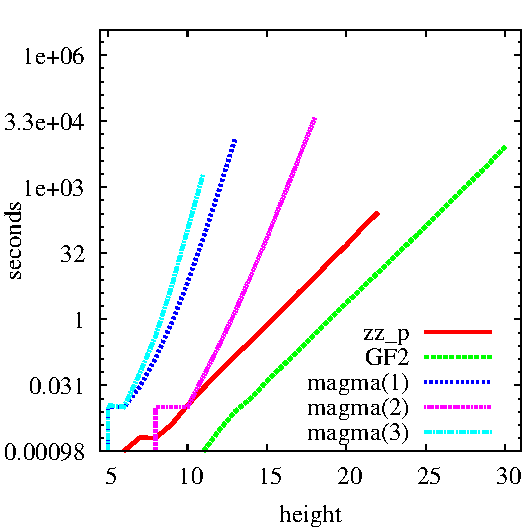
\includegraphics[height=0.5\textwidth]{artin/build1}
  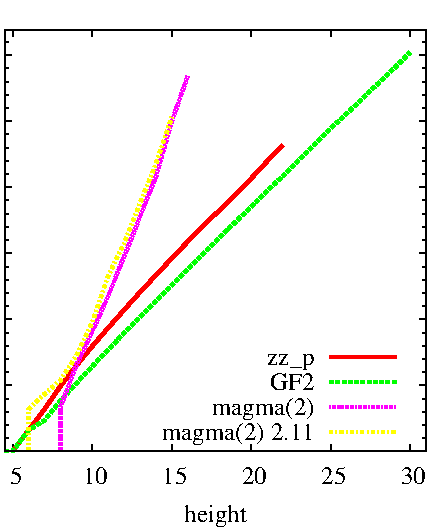
\includegraphics[height=0.5\textwidth]{artin/iso1}
  
  \caption{Build time (left) and isomorphism time (right) with respect to tower height. Plot is in logarithmic scale.}
  \label{fig:height}
\end{figure}

\begin{figure}
  \centering
  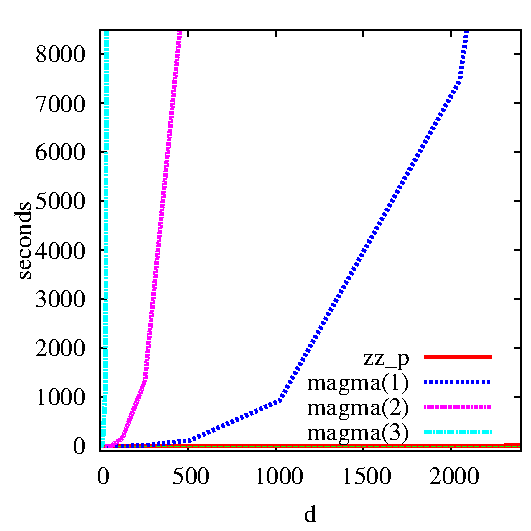
\includegraphics[height=0.5\textwidth]{artin/build-d}
  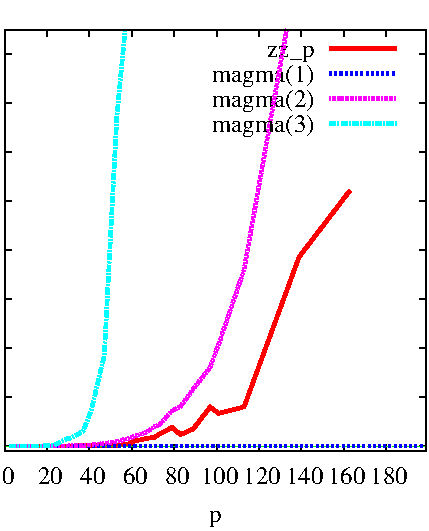
\includegraphics[height=0.5\textwidth]{artin/build-p}
  
  \caption{Build times with respect to $d$ (left) and $p$ (right).}
  \label{fig:p-d}
\end{figure}

\pdfmcthree{A little comment on magma(2) for p increasing.}
The timings of our code are significantly better for increasing height
or increasing $d$. Not surprisingly, for increasing $p$, the magma(1)
approach performs better than any other: the \texttt{quo} operation
simply creates a residue class ring, regardless of the
(ir)reducibility of the modulus, so the timing for building two levels
barely depend on $p$. The most adapted approach for this situation
presumably is magma(2); yet we notice that \texttt{FAAST} has
reasonable performances for characteristics up to about $p=50$.

In Tables~\ref{tab:arith-gf2} and~\ref{tab:arith-zzp} we provide some
comparative timings for the different arithmetic operations provided
by \texttt{FAAST}. The column ``Primitive'' gives the time taken to
build one level of the primitive tower (this includes the
precomputation of the data as described in
Subsection~\ref{sec:level-embedding:lift-up}); the other entries are
self-explanatory. Product and inversion are just wrappers around
\texttt{NTL} routines: in these operations we did not observe any
overhead compared to the native \texttt{NTL} code. All the operations
stay within a factor of $30$ of the cost of multiplication, which is
satisfactory.

\begin{table}
  \centering
  \begin{tabular}{l r r r r r r r}
    \hline
    \small level & \small Primitive & \small Push-d. & \small Lift-up & \small Product & \small Reciprocal & \small apply $\sigma^{-1}$ & \small apply $\sigma$ \\
    \hline
    19 &  1.143 & 0.304 &  1.265 & 0.039 &  0.649 &  0.652 &  1.290\\
    20 &  2.566 & 0.609 &  2.796 & 0.081 &  1.544 &  1.314 &  2.602\\
    21 &  5.686 & 1.225 &  6.147 & 0.187 &  3.598 &  2.409 &  2.668\\
    22 & 12.660 & 2.515 & 13.746 & 0.463 &  8.355 &  5.565 & 11.179\\
    23 & 28.511 & 5.295 & 31.200 & 1.046 & 19.522 & 12.323 & 24.740
  \end{tabular}
  \caption{Some timings in seconds for arithmetics in a generic tower built over $\F_2$ using \texttt{GF2}.}
  \label{tab:arith-gf2}
\end{table}

\begin{table}
  \centering
  \begin{tabular}{l r r r r r r r}
    \hline
    \small level & \small Primitive & \small Push-d. & \small Lift-up & \small Product & \small Reciprocal & \small $\sigma^{-1}$ & \small  $\sigma$ \\
    \hline
    18 &  13.618 &  0.884 &  13.712 & 0.476 &  10.753 &  1.337 &  3.578\\
    19 &  30.288 &  1.814 &  30.432 & 1.001 &  23.046 &  2.850 &  7.798\\
    20 &  65.632 &  3.953 &  66.889 & 2.106 &  51.544 &  6.564 & 18.141\\
    21 & 128.190 &  8.347 & 131.271 & 4.791 & 121.349 & 14.396 & 39.296\\
    22 & 296.671 & 11.396 & 298.541 & 6.413 & 249.520 & 28.851 & 86.628
  \end{tabular}
  \caption{Some timings in seconds for arithmetics in a generic tower built over $\F_2$ using \texttt{zz\_p}.}
  \label{tab:arith-zzp}
\end{table}


Finally, we mention the cost of precomputation. The precomputation of
the images of $\sigma$ as explained in
Section~\ref{sec:couveignes-algorithm} is quite expensive; most of it
is spent computing pseudotraces. Indeed it took one week to precompute
the data in Figure~\ref{fig:height} (right), while all the other data
can be computed in a few hours. There is still space for some minor
improvement in \texttt{FAAST}, mainly tweaking recursion thresholds
and implementing better algorithms for small and moderate input
sizes. Yet we think that only a major algorithmic improvement could
consistently speed up this phase.



% Local Variables: 
% mode:flyspell
% ispell-local-dictionary:"american"
% TeX-master: "../these"
% mode: TeX-PDF
% mode: reftex
% End: 
%
% LocalWords:  univariate isogeny Couveignes isogenies Artin Schreier



% Local Variables:
% mode:flyspell
% ispell-local-dictionary:"american"
% mode:TeX-PDF
% mode:reftex
% TeX-master: "../these"
% End:
